\chapter{Evaluation}
\label{sec:evaluation}

The articulated tracking approach and the incorporation of prior information is evaluated on two different data sets. The data set for the \textit{first experiment} contains depth observations from a manipulator that is moving close to a table and an object. This experiment will be used to compare different approaches to incorporate prior information in the tracking process.

The data set for the \textit{second experiment} contains stereo camera observations of the manipulator at different viewing angles without nearby objects. This data set additionally contains ground truth hand poses that were measured by the Vicon system. The main purpose of this experiment is the comparison of the estimated hand pose with the measured ground truth.

\section{Experiment 1: Incorporating Prior Information}

This section will evaluate the application of prior information in a setting where a robot hand moves close to an object and a table. Two sources of depth information are considered: enhanced stereo matching using IR dot projection (denoted as \emph{stereo}) and structured light (denoted as \emph{xtion} as in Asus Xtion).

\subsection{Hypotheses}

In the base implementation of the assessed tracking approach, its gradient is determined by the signed distance function. Hence, the optimization is driven by the observation once the iteration is initialized with the reported state. Using additional information that effects the gradient can improve the state estimation by driving it away from distracting observations.

\begin{hypothesis}(Distracting sensor readings)\\
Distracting sensor readings will impair the tracking performance of the manipulator.
\label{hyp:distracting_readings}
\end{hypothesis}

\begin{hypothesis}(Use of prior information)\\
Using prior information will reduce the negative effects of distracting sensor readings. Increasing weights will further decrease the dependency on the sensor readings.
\label{hyp:prior_information}
\end{hypothesis}


\subsection{Setup}

A robot was placed in front of a table with a bottle on it. The left hand was moved from close to the table plane towards the object. Once the object is pushed, the hand moved up and back to its initial position.
The setup, as it is perceived by the robots stereo vision in the initial state, is shown in \cref{fig:exp1_setup}.

%\begin{figure}
%\centering
%\begin{minipage}{0.45\textwidth}
%\centering
%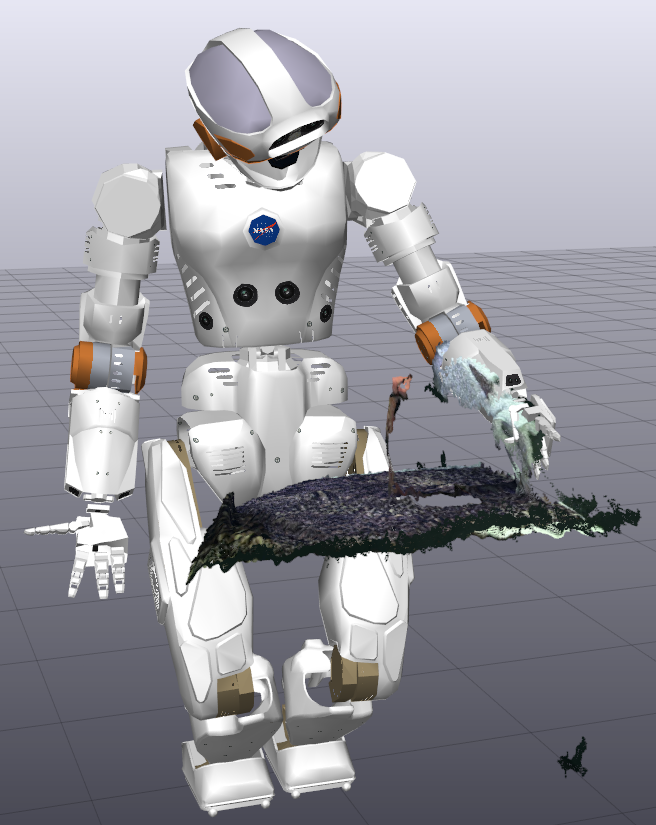
\includegraphics[width=1.0\textwidth]{images/eval_prior/sequence/prior_setting.png} 
%\caption{Joint prior setup}
%\label{fig:prior_setting}
%\end{minipage}
%%
%\hspace{0.3cm}
%\begin{minipage}{0.45\textwidth}
%\vspace{0.8cm}
%\centering
%\subfloat[start (t=0)]{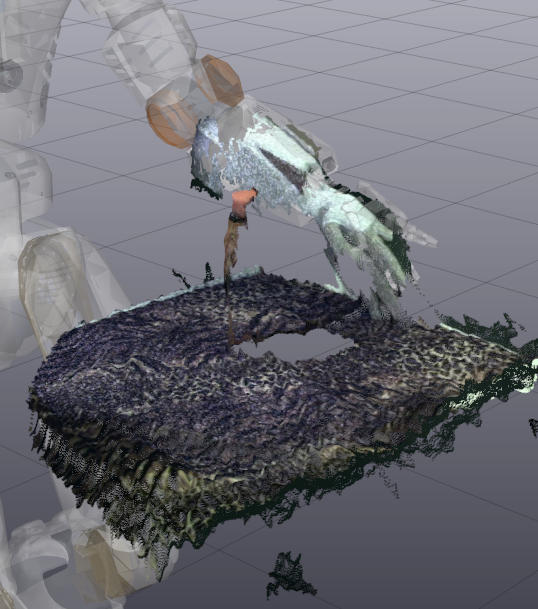
\includegraphics[width=0.5\textwidth]{images/eval_prior/sequence/bottle_0_init.png} \label{fig:prior_movement_phases_start}}
%\subfloat[moved upwards (t=10)]{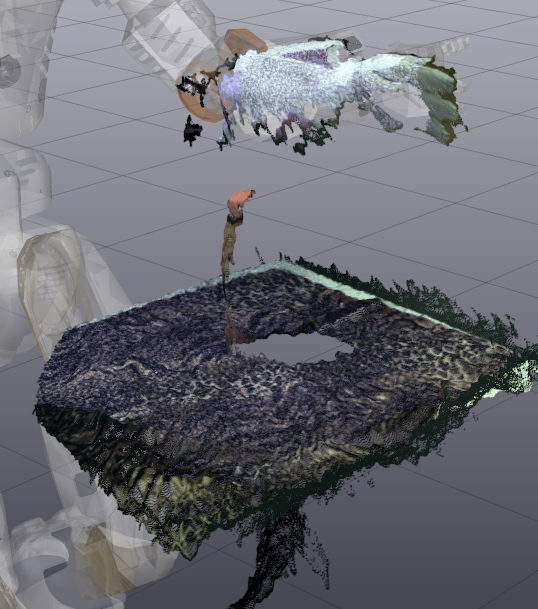
\includegraphics[width=0.5\textwidth]{images/eval_prior/sequence/bottle_10_up.png} }
%
%\subfloat[object contact (t=22)]{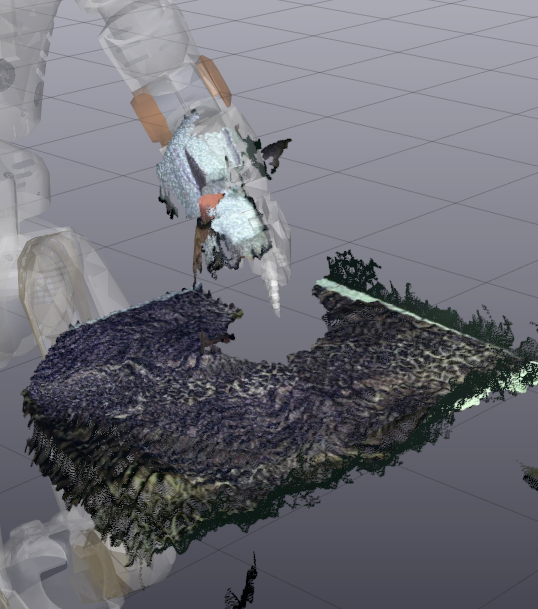
\includegraphics[width=0.5\textwidth]{images/eval_prior/sequence/bottle_22_object.png} 
%\label{fig:prior_movement_phases_contact}}
%\subfloat[end (t=35)]{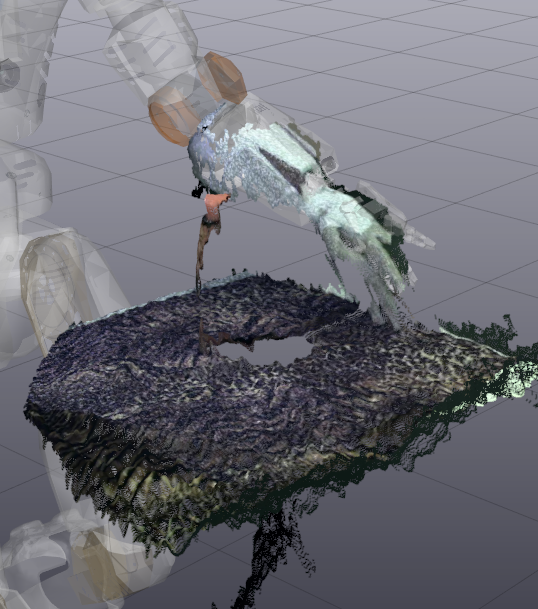
\includegraphics[width=0.5\textwidth]{images/eval_prior/sequence/bottle_35_end.png} }
%\caption[States between movements]{Sequence of states between movements (time in seconds)}
%\label{fig:prior_movement_phases}
%\end{minipage}
%\end{figure}


\begin{figure}[h]
\centering
\subfloat[Point cloud and reported robot state]{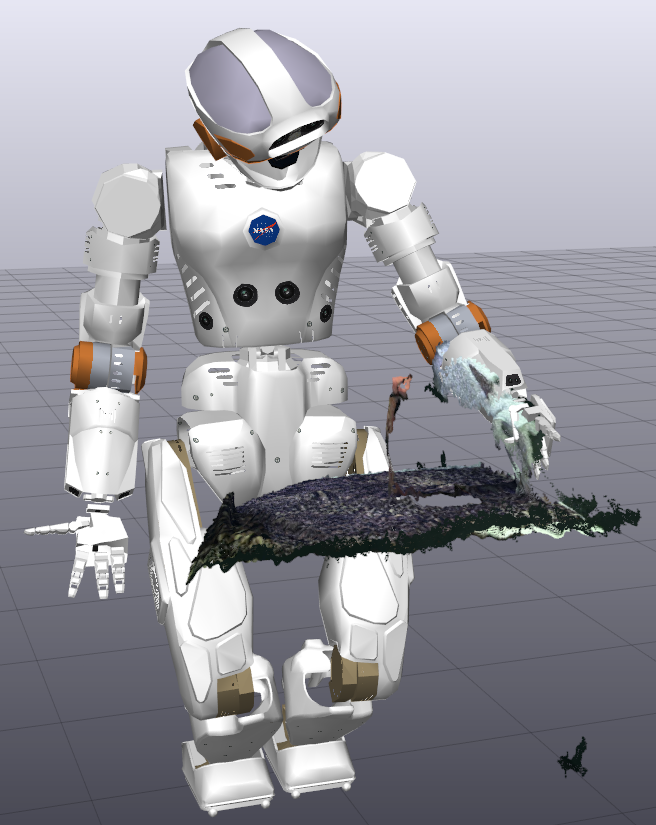
\includegraphics[height=7cm]{images/eval_prior/sequence/prior_setting.png} }
\hspace{1cm}
\subfloat[View from left camera]{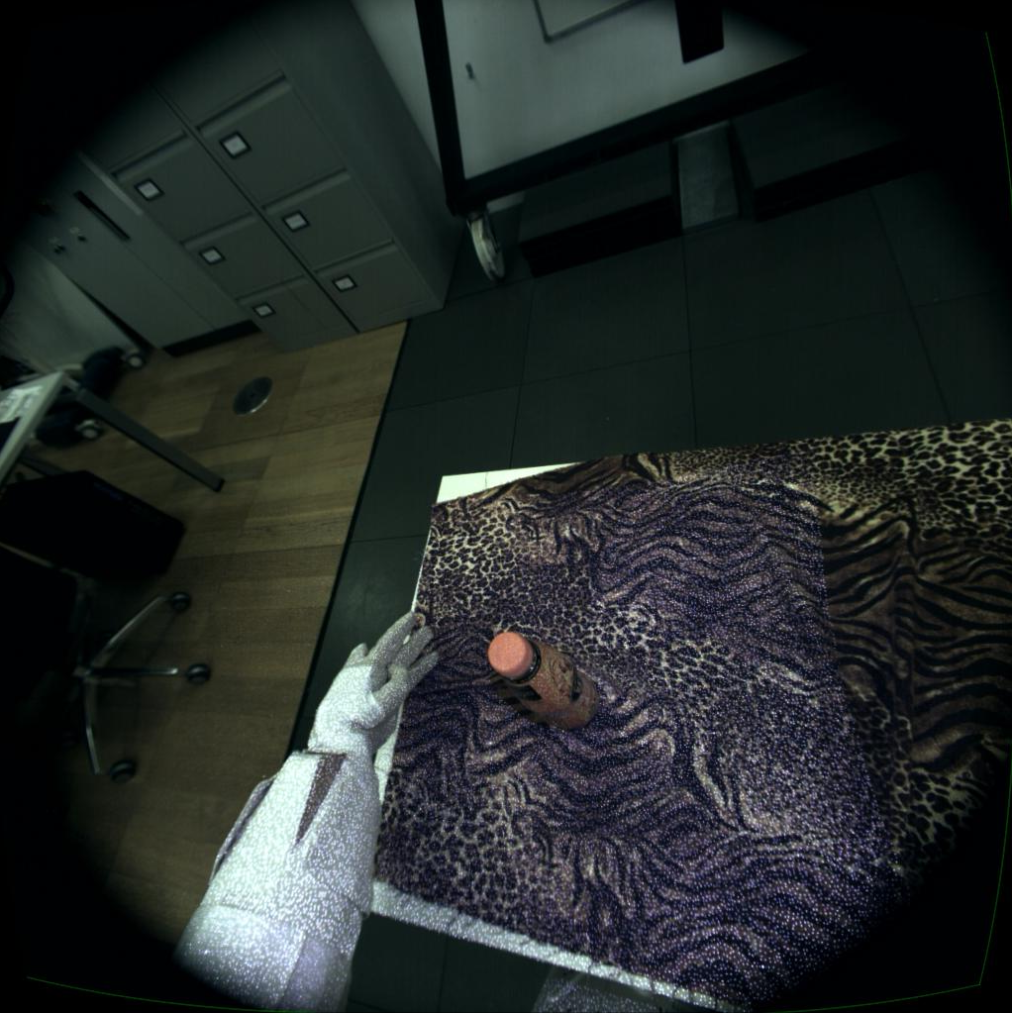
\includegraphics[height=7cm]{images/eval_prior/sequence/camera_view_initial.png} }
\caption[Experiment 1: Setup]{Experiment 1: Setup with robot in front of table. Initial state where manipulator is observed close to table plane.}
\label{fig:exp1_setup}
\end{figure}

The motion sequence is divided into 5 states which change by 4 movements. The movement phases are defined in \cref{tab:prior_movement_phases}. Two of the phases define movements of the manipulator away from objects after being in contact with them. These phases are highlighted in the table and in the plots.

\begin{table}[h]
\centering
\begin{tabular}{|c|l|l|}
\hline
 & \emph{time (s)} & \emph{movement description} \\
\hline
1 & 0$\dots$3 & arm resting on table \\
\hline
\rowcolor{gray!30} \textbf{2} & 3$\dots$10 & upward from table \\
\hline
3 & 10$\dots$20 & towards object \\
\hline
\rowcolor{gray!30} \textbf{4} & 20$\dots$30 & away from object \\
\hline
5 & 30$\dots$35 & downward towards table \\
\hline
\end{tabular}
\caption{Phases of arm movement in experiment 1. Highlighted rows emphasise movements away from objects like the table or bottle.}
\label{tab:prior_movement_phases}
\end{table}

The perceived point cloud of the first three states and the final state are shown in \cref{fig:prior_movement_phases}.
Especially the movement phases 2 and 4, respectively movements starting in states shown in \cref{fig:prior_movement_phases_start,fig:prior_movement_phases_contact} are of interest.

\begin{figure}[h]
\centering
\subfloat[start (t=0)]{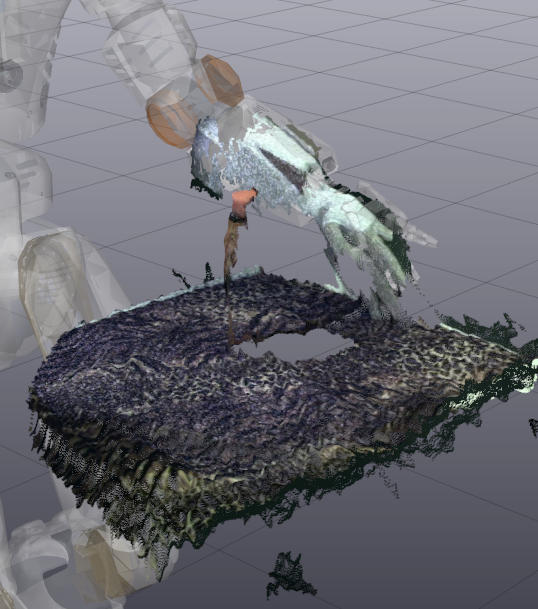
\includegraphics[width=0.25\textwidth]{images/eval_prior/sequence/bottle_0_init.png} \label{fig:prior_movement_phases_start}}
\subfloat[moved upwards (t=10)]{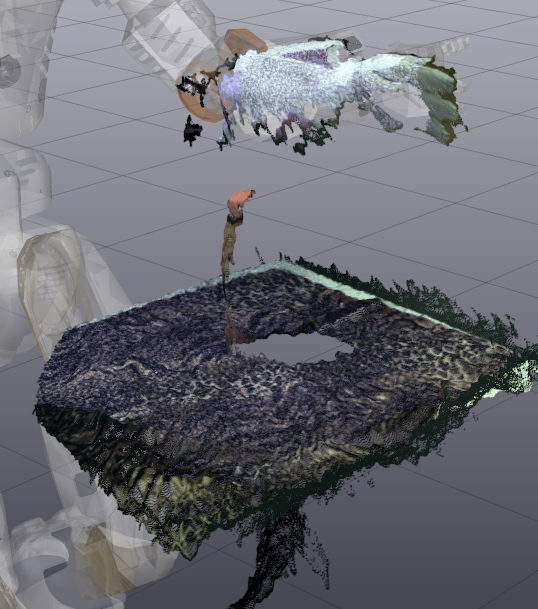
\includegraphics[width=0.25\textwidth]{images/eval_prior/sequence/bottle_10_up.png} }
\subfloat[object contact (t=22)]{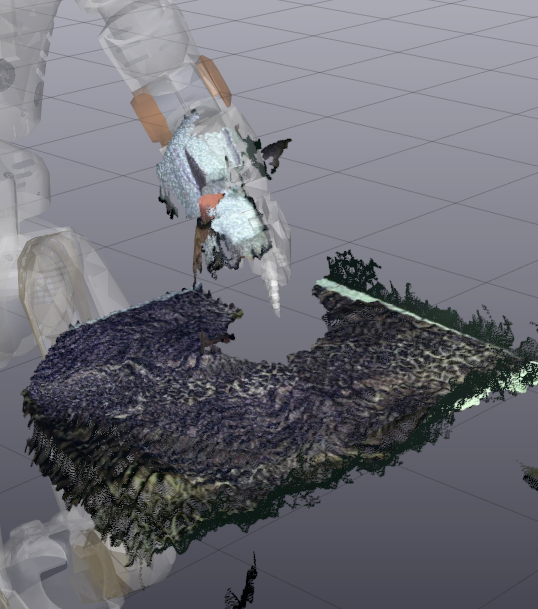
\includegraphics[width=0.25\textwidth]{images/eval_prior/sequence/bottle_22_object.png} 
\label{fig:prior_movement_phases_contact}}
\subfloat[end (t=35)]{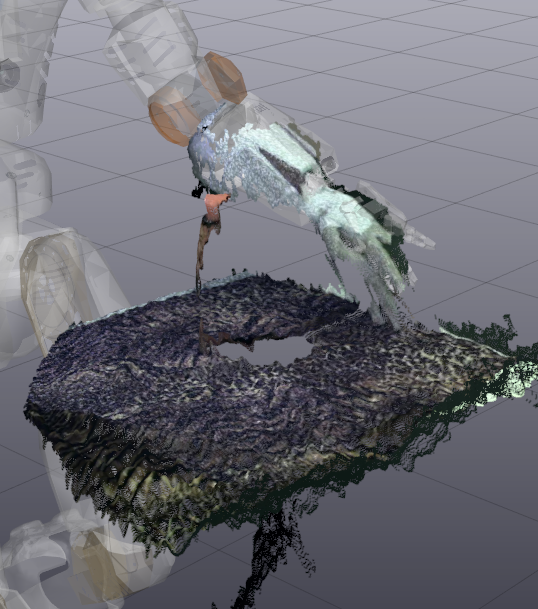
\includegraphics[width=0.25\textwidth]{images/eval_prior/sequence/bottle_35_end.png} }
\caption[Experiment 1: States between movements]{Sequence of states between movements in experiment 1 (time in seconds)}
\label{fig:prior_movement_phases}
\end{figure}

During the movement, depth data is collected simultaneously from the MultiSense stereo sensor and the Asus Xtion structured light sensor. Hence, the stereo block matching benefits from the distinctive IR dots.


\subsection{Results}
\label{sec:prior_results}

For this experiment, we are interested in the deviation of the estimated state from the reported state. This will allow us to (1) see how the estimation on the observed point cloud is deviating from its initial reported pose, and (2) investigate the effect of the prior objective compared to the base signed distance objective. We will refer to this deviation as \emph{error}.

The error in joint and task space is computed as L2 norm (Euclidean distance) of its components and plotted over time. In joint space these components are the left fingers (13 DoF: 3 $\times$ \emph{leftIndexFingerPitch}, 3 $\times$ \emph{leftMiddleFingerPitch}, 3 $\times$ \emph{leftPinkyPitch}, 3 $\times$ \emph{leftThumbPitch} and 1 $\times$ \emph{leftThumbRoll}) and the left arm (7 DoF: \emph{leftShoulderPitch/Roll/Yaw}, \emph{leftElbowPitch}, \emph{leftForearmYaw}, \emph{leftWristRoll/Pitch}). In task space, the 3D position ($x,y,z$) and the 3D orientation (\textit{roll}, \textit{pitch}, \textit{yaw}) of the left hand (frame: \emph{leftPalm}) are computed via forward kinematics on the reported and estimated robot configuration.

\subsubsection{Joint Prior Objective with Common Weight}

The following plots compare the joint and task space errors for the two depth sources for common weights in the range 0 to 5. The common weighting scheme \emph{Weighted L2 norm of joint position deviation} (objective function \cref{eqn:objf_weightedL2}) is applied. A weight of 0 indicates that no prior is used at all.

\paragraph{Stereo}

\Cref{fig:stereo_joint_error} compares the joint space error for left fingers and arm. For both parts, after the optimization reaches the steady state, the maximum error is reached when no prior information from the reported configuration is used. In this case, the configuration is solely optimized using the distance to the observed point cloud. If the manipulator is close to a large concentration of points, the optimization will relate these readings to the manipulator (\cref{fig:no_prior_fingers_table}).
The general trend is that the error decreases with increasing weight. This is not true for the arm movement in the second half of phase 4 ($t=[20,30]$), where weights of $0.2$ and $0.5$ result in larger errors compared to no prior.

The largest decrease in error can be seen for the finger joints when using already a small weight of $0.2$. A similar effect is not present for the arm joints. This is presumably because the robot can only observe the lower part of its arm and hence the arm configuration is mostly determined by its initial state close to the reported state.

\begin{SCfigure}
\centering
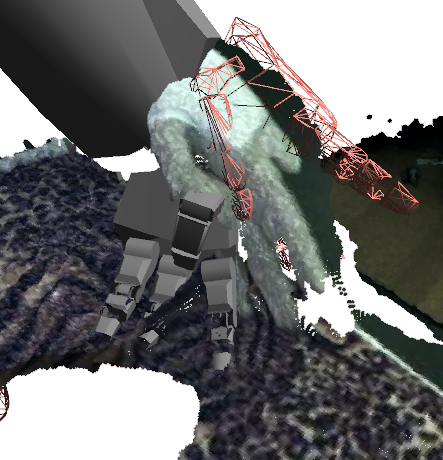
\includegraphics[width=0.5\textwidth]{images/eval_prior/fingers_in_table.png}
\caption[Wrong association of data points]{Close points from the table plane are associated to the fingers (solid gray mesh). Using solely the signed distance as objective, the gradient based optimization finds a local minimum in regions with dense sensor readings close the initial reported state (red wired mesh).}
\label{fig:no_prior_fingers_table}
\end{SCfigure}

\begin{figure}[h]
\centering
\subfloat[finger joints]{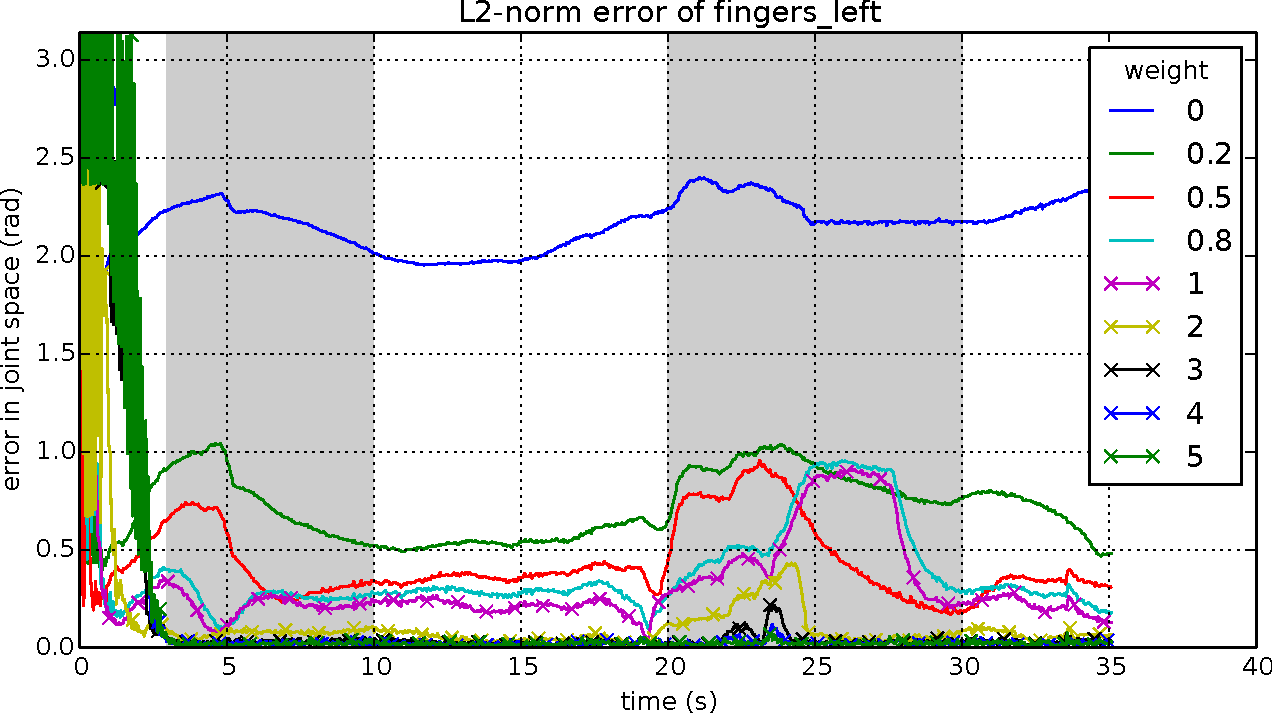
\includegraphics[width=0.5\textwidth]{images/eval_prior/common_weights/stereo_finger_joint_error.pdf} \label{fig:stereo_joint_error_hand} }
%
\subfloat[arm joints]{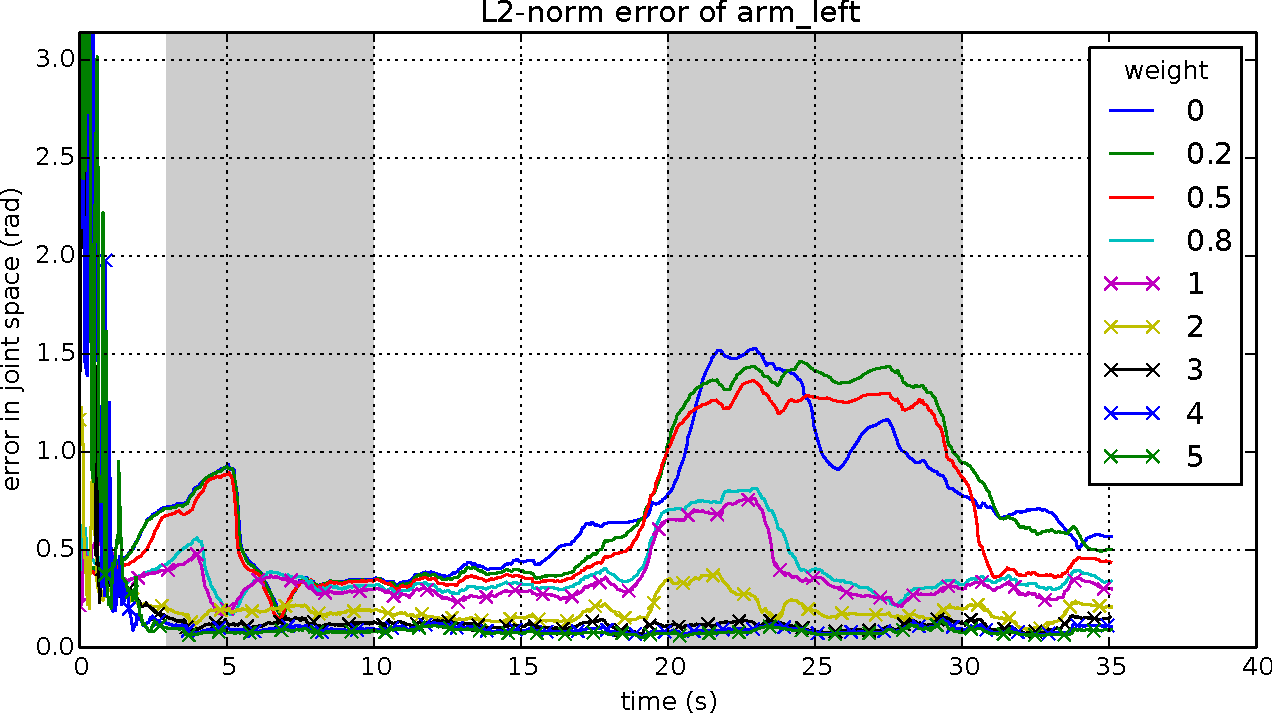
\includegraphics[width=0.5\textwidth]{images/eval_prior/common_weights/stereo_arm_joint_error.pdf} \label{fig:stereo_joint_error_arm} }
\caption[Joint space error (Exp. 1, stereo)]{Joint space error for finger and arm joints (Exp. 1, \textit{stereo} data). The finger joint deviation (a) can already be reduced by a weak bias towards the reported pose ($0.2$, $0.5$), while the arm joints (b) require a higher weight ($\geq0.8$).}
\label{fig:stereo_joint_error}
\end{figure}

As the hand position and orientation only depends on the arm configuration but not the finger configuration, we expect some relation between the joint error of the arm and the pose error on the hand frame. We can see this relation, when comparing the joint space error for the arm in \cref{fig:stereo_joint_error_arm} and the hand pose error in \cref{fig:stereo_hand_pose_error}. In particular the error increases in phases where the hand moves upwards and when it moves away from the object (phases 2 and 4). The position error can be reduced significantly when using a prior with low weight ($0.2$), whereas the orientation error reduces only when using prior weights larger or equal than $0.8$.

\begin{figure}[h]
\centering
\subfloat[position error]{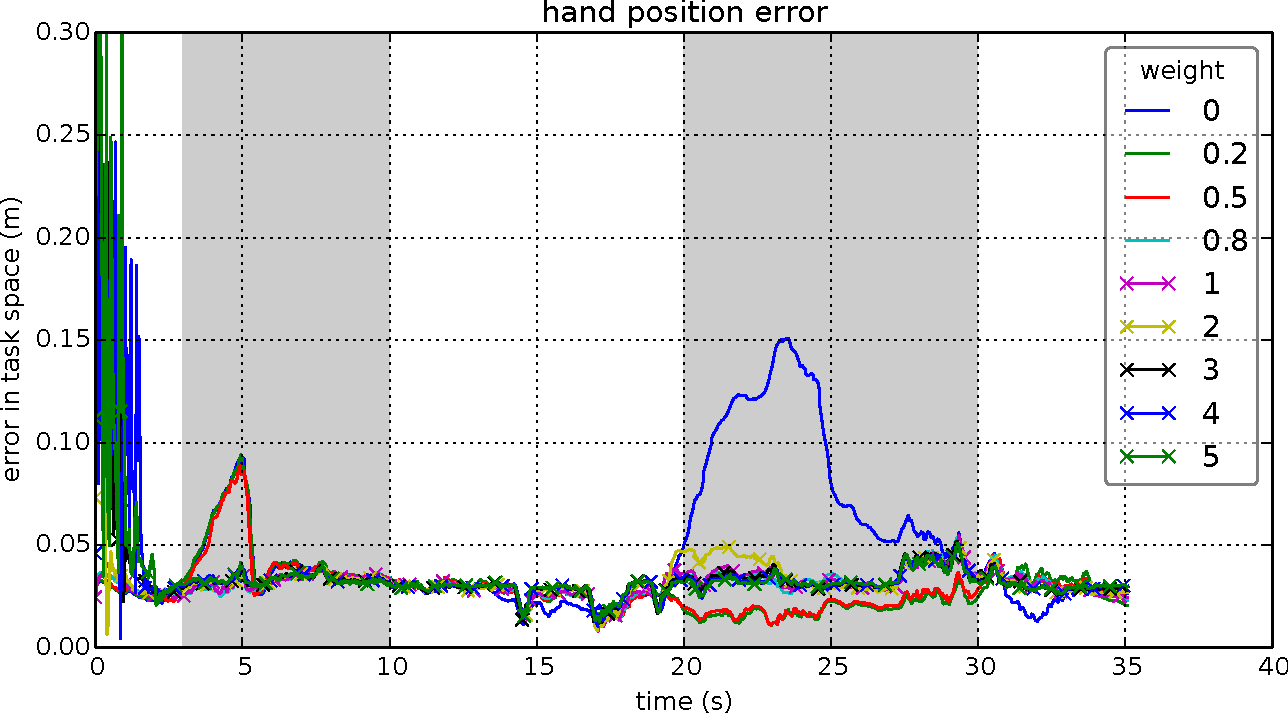
\includegraphics[width=0.5\textwidth]{images/eval_prior/common_weights/stereo_hand_pos_error.pdf} \label{fig:stereo_hand_pos_error}}
%
\subfloat[orientation error]{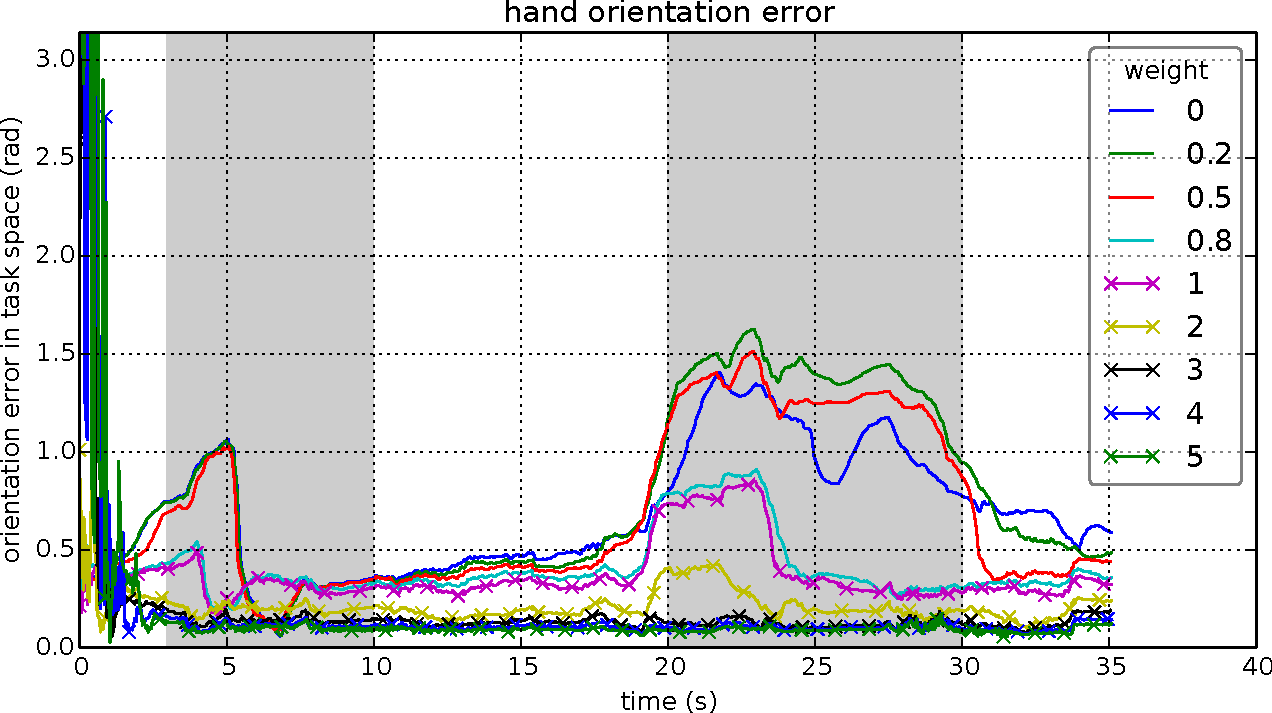
\includegraphics[width=0.5\textwidth]{images/eval_prior/common_weights/stereo_hand_ori_error.pdf}
\label{fig:stereo_hand_ori_error}}
\caption[Task space error (Exp. 1, stereo)]{Task space error for left hand pose (Exp. 1, \textit{stereo} data). (a) The hand position error can already be reduced by minimal weighting of the prior objective. (b) Small weights actually increase the error and higher weights of at least $0.8$ are required to enforce the reported pose.}
\label{fig:stereo_hand_pose_error}
\end{figure}


\paragraph{Asus Xtion}

Using the structured light sensor Asus Xtion, the behaviour of decreasing error with increasing weight is comparable to that seen for the stereo matching sensor. Similar to the stereo sensor (\cref{fig:stereo_joint_error_hand}), the error on the finger joints reduces significantly when using a small weight of $0.2$ (\cref{fig:xtion_joint_error_hand}).
In contrast to the small errors on the arm joints when using stereo in the phase of moving towards the object (\cref{fig:stereo_joint_error_arm}), the error in this phase when using the Xtion sensor is fairly large for no and low weighted prior (\cref{fig:xtion_joint_error_arm}).

\begin{figure}[h]
\centering
\subfloat[finger joints]{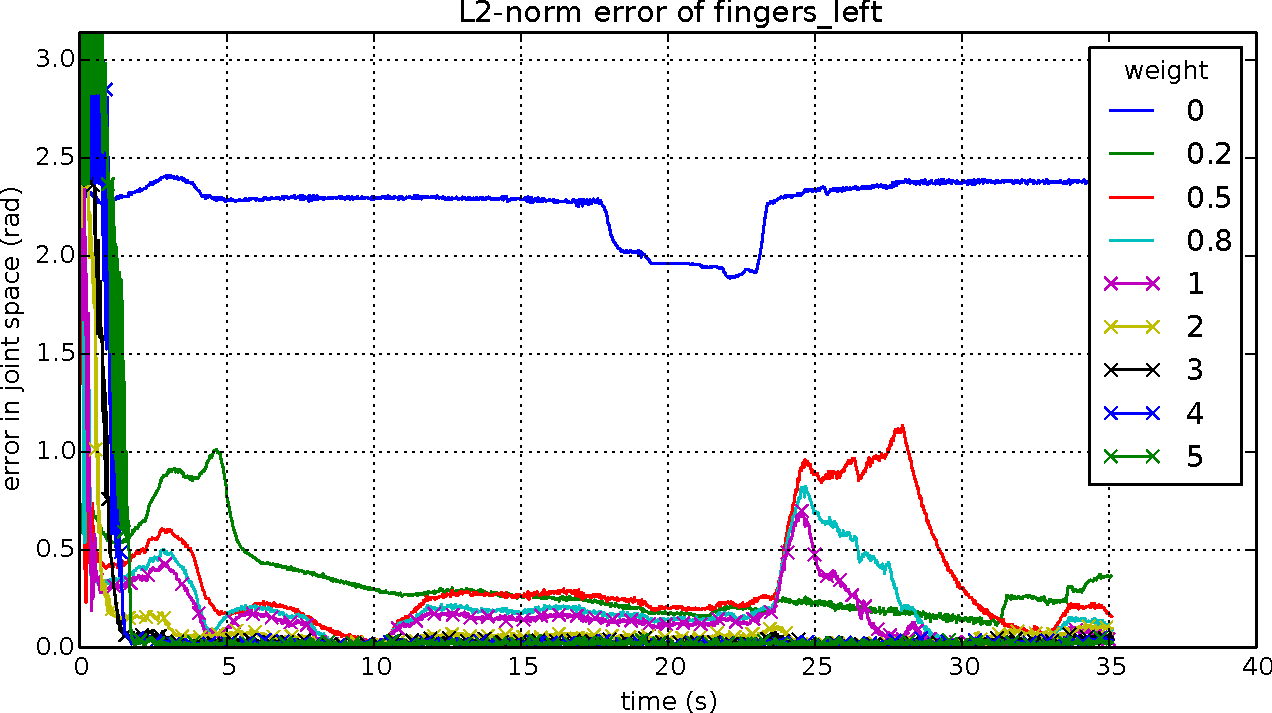
\includegraphics[width=0.5\textwidth]{images/eval_prior/common_weights/xtion_finger_joint_error.pdf} \label{fig:xtion_joint_error_hand}}
%
\subfloat[arm joints]{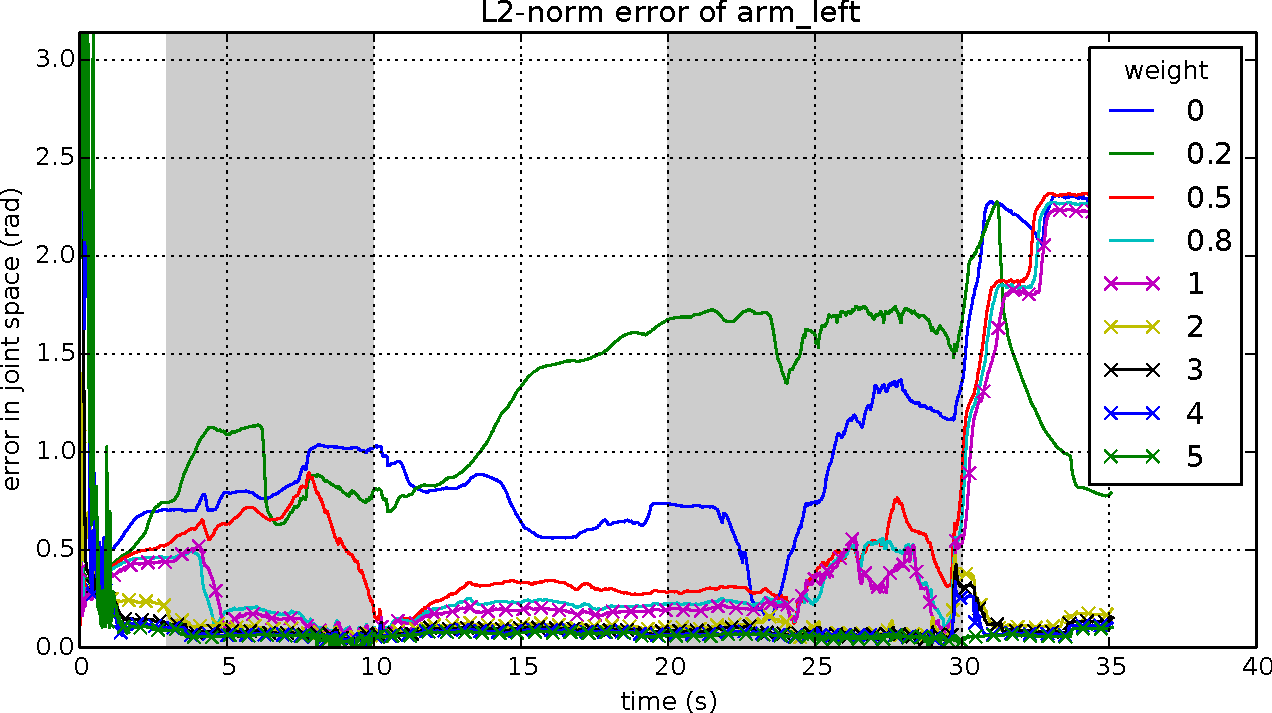
\includegraphics[width=0.5\textwidth]{images/eval_prior/common_weights/xtion_arm_joint_error.pdf} \label{fig:xtion_joint_error_arm}}
\caption[Joint space error (Exp. 1, xtion)]{Joint space error for finger and arm joints (Exp. 1, \textit{xtion} data). Comparable to stereo data set, the finger joint deviation (a) is already reduced by small weights.}
\label{fig:xtion_joint_error}
\end{figure}

As before, the hand pose error is only effected by the arm joint errors and thus the hand position error shown in \cref{fig:xtion_hand_pos_error} is large in the same moving phase close to the object. For using the structured light sensor, a common weight of at least $2$ is required to drive the solution towards the reported hand position.

\begin{figure}[h]
\centering
\subfloat[position error]{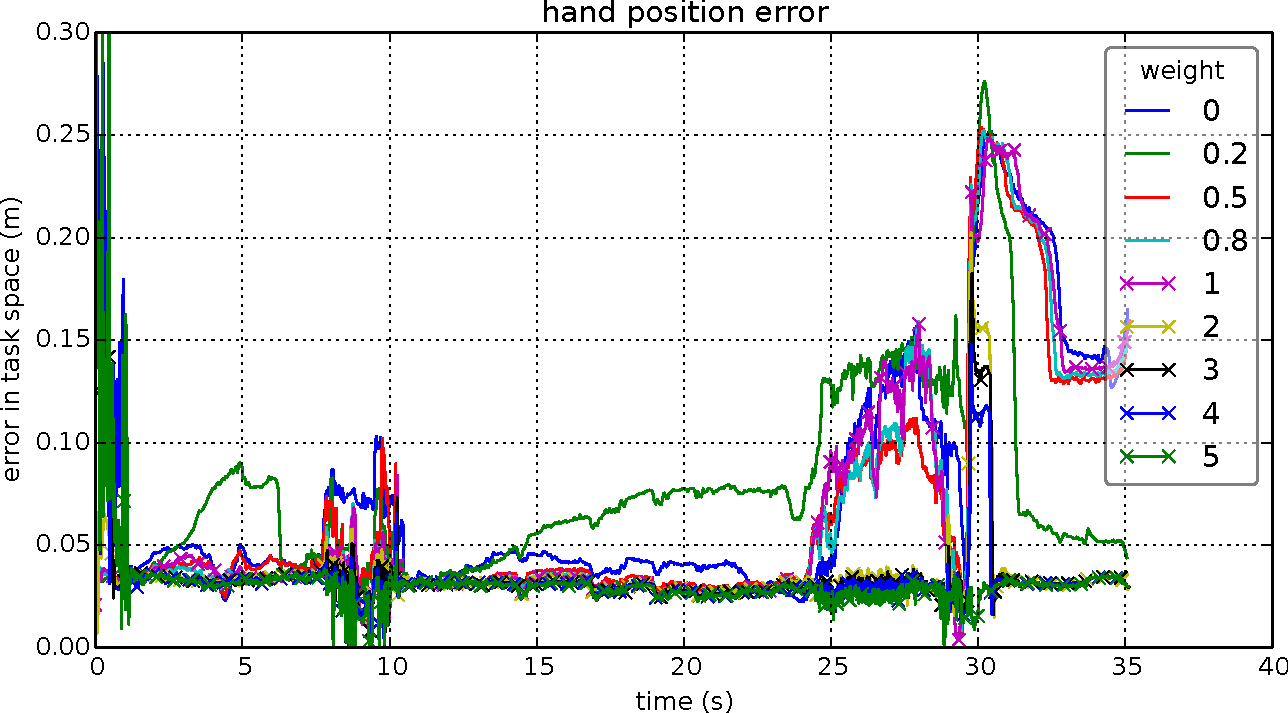
\includegraphics[width=0.5\textwidth]{images/eval_prior/common_weights/xtion_hand_pos_error.pdf} \label{fig:xtion_hand_pos_error}}
%
\subfloat[orientation error]{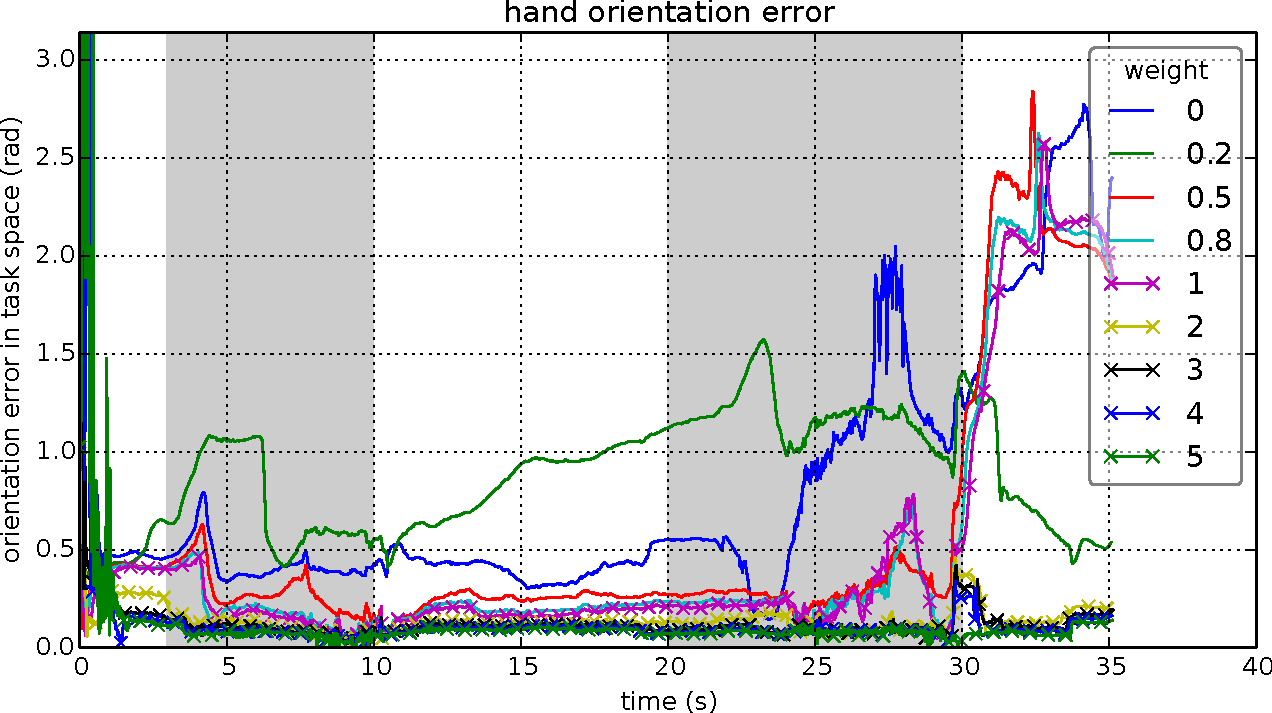
\includegraphics[width=0.5\textwidth]{images/eval_prior/common_weights/xtion_hand_ori_error.pdf} \label{fig:xtion_hand_ori_error}}
\caption[Task space error (Exp. 1, xtion)]{Task space error for left hand pose (Exp. 1, \textit{xtion} data). The pose error on this data set has a different characteristic than on the stereo data set. Large weights above $2$ are required to enforce the reported pose.}
\label{fig:xtion_hand_pose_error}
\end{figure}

\subsubsection{Joint Prior Objective with Individual Weights}

Individual weighting is applied to stereo depth data only. This weighting scheme enables us to weight each combination of joint deviations separately as defined by \cref{eqn:objf_indiv_weighted}. For simplicity, only single joint deviations are weighted. That is, the weight matrix $Q$ will be a diagonal matrix where only the diagonal elements $q_{i,i}$ will be defined.

In this scenario, the two palm joints (\texttt{leftWristRoll} and \texttt{leftWristPitch}) that connect the hand with the arm are weighted with increasing weights, while the remaining joints are kept constant at either low weights ($0.2$ for finger joints, $0.2$ for remaining joints) or kept constant at normal weights ($0.2$ for finger joints, $1.0$ for remaining joints).

%In this scenario, three setting of joints are weighted and this scheme is captured in the legend as follows: first, all diagonal elements of $Q$ are set to the weight \emph{q}, second, the 13 finger joints are set to the weight \emph{fingers} and optionally third, the two palm joints (\texttt{leftWristRoll} and \texttt{leftWristPitch}) are set to the value \emph{palm}. E.g., a plot named "\texttt{q 1, fingers 0.2, palm 5}" indicates that finger joints in the diagonal are weighted by $0.2$, palm joints are weighted with $5$ and the remaining joints are weighted with $1$.

%\Cref{fig:indiv_joint_error} shows the joint space error for fingers and arms separately as before.

Because we specifically weight both palm joints, the joint space error of the finger and the arm joints are effected in different ways (\cref{fig:indiv_joint_error}). While the arm joint error reduces with increasing palm weight, the finger joint error actually increases. The reason for this is that both palm joints, as part of the arm kinematic chain, determine the pose of the hand palm. While the hand pose is biased towards the reported pose by the prior, the fingers do not benefit from this prior information to the same extent.


%From these plots we can see that the individual weighting affects the fingers and the arm in different ways. The finger joint error in \cref{fig:indiv_joint_error_hand} shows that, raising the palm weights and keeping the remaining constant, actually impairs the performance (e.g., compare "\texttt{q 1, fingers 0.2}" with palm weights raised from \texttt{palm 1} to \texttt{palm 5}). In contrast to this, the arm joint error is reduced when increasing the palm weights and keeping remaining weights constant (e.g., compare \texttt{q 0.2, fingers 0.2, palm 5} and palm weights raised to \texttt{q 0.2, fingers 0.2, palm 25}).

\begin{figure}[h]
\centering
\subfloat[finger joints]{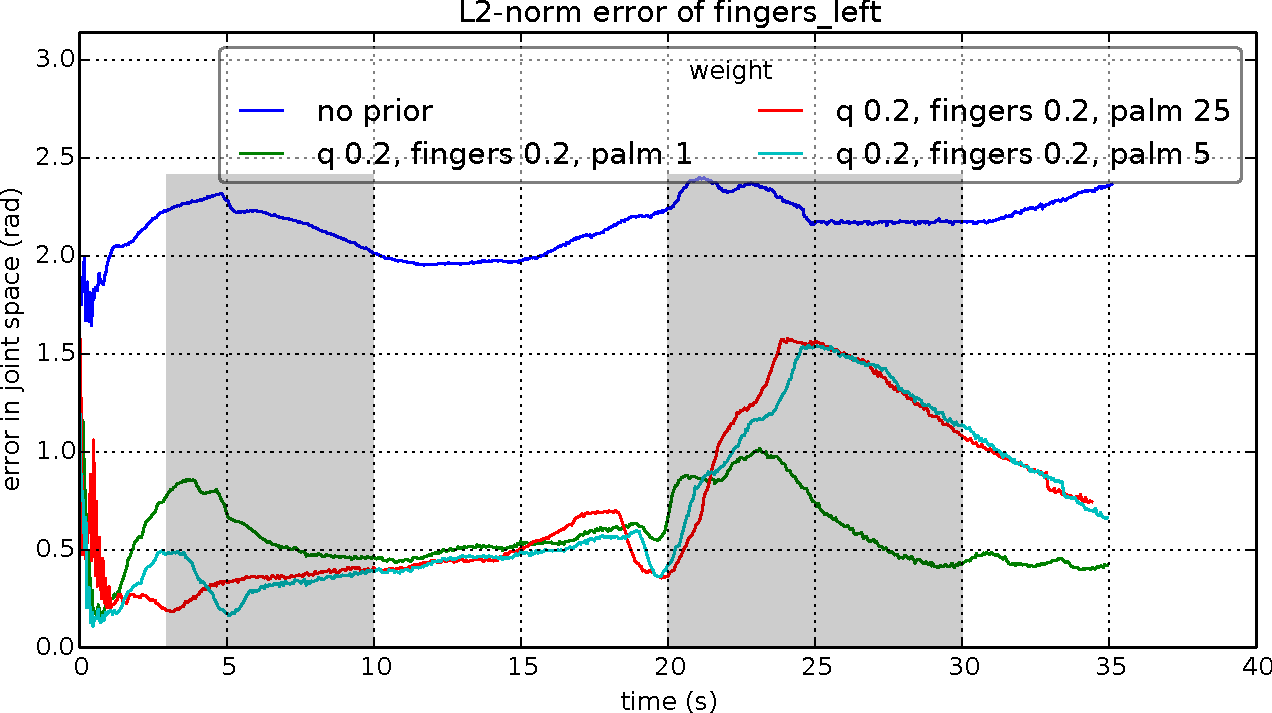
\includegraphics[width=0.5\textwidth]{images/eval_prior/inidv_weights/q0_stereo_finger_joint_error.pdf} }
%
\subfloat[arm joints]{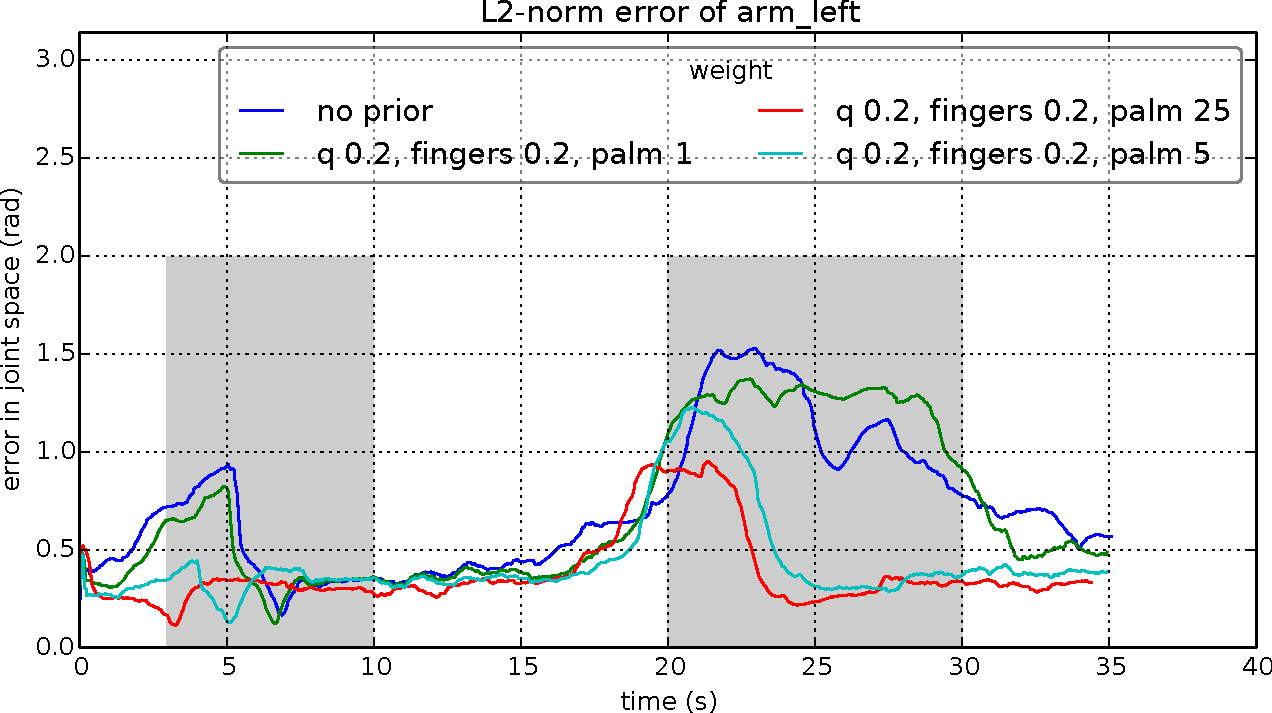
\includegraphics[width=0.5\textwidth]{images/eval_prior/inidv_weights/q0_stereo_arm_joint_error.pdf} }

\subfloat[finger joints]{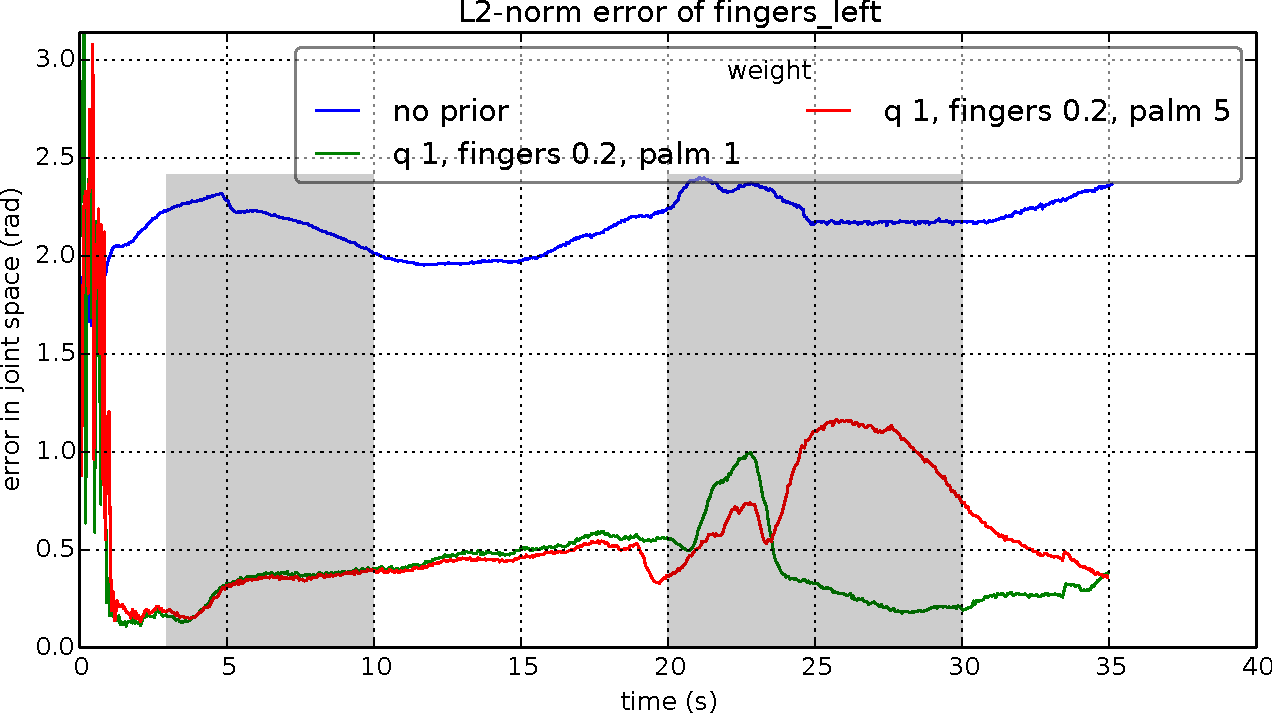
\includegraphics[width=0.5\textwidth]{images/eval_prior/inidv_weights/q1_stereo_finger_joint_error.pdf} }
%
\subfloat[arm joints]{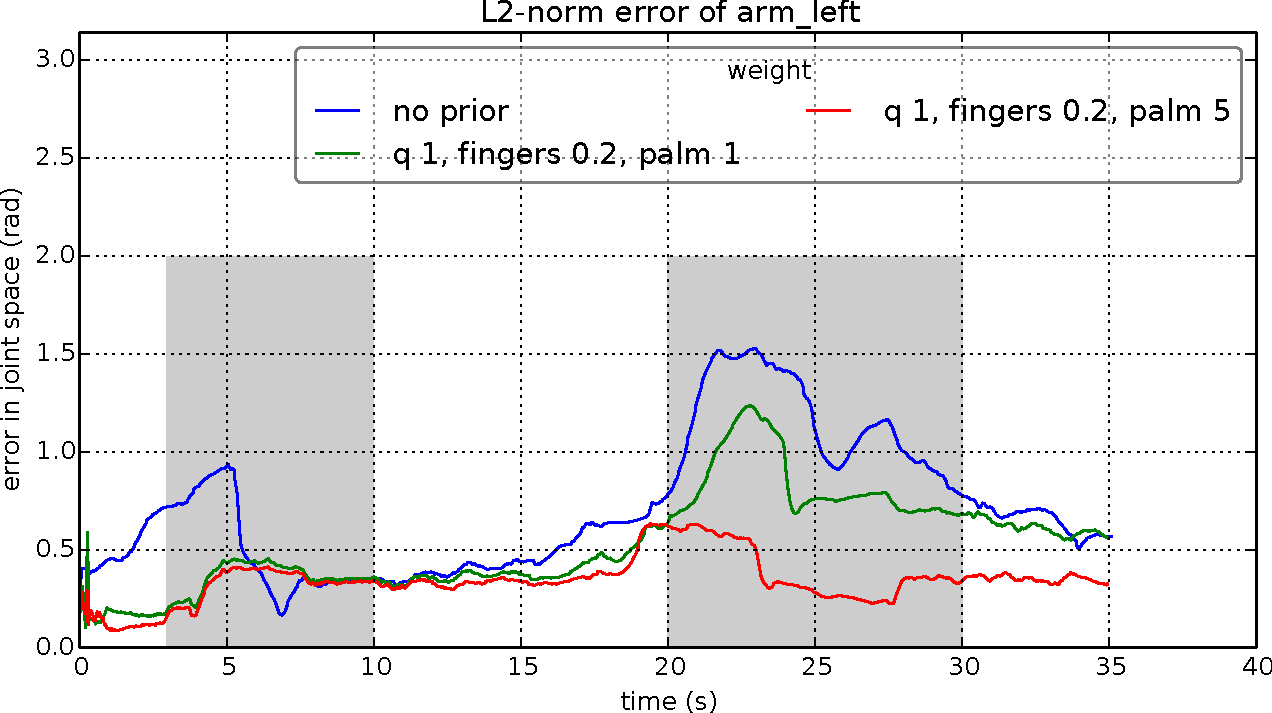
\includegraphics[width=0.5\textwidth]{images/eval_prior/inidv_weights/q1_stereo_arm_joint_error.pdf} }

\caption[Joint space error for individual weighting (Exp. 1)]{Joint space error for individual weighting (Exp. 1). Weights on palm joints are increased ($1$, $5$, $25$) while remaining joints are kept constant at low weights (a,b) or at normal weights (c,d). Finger joint errors (a,c) increase with increasing palm weights, while arm joint errors (b,d) are reduced.}
\label{fig:indiv_joint_error}
\end{figure}

%Again, the arm joints directly influence the pose error of the hand as seen in \cref{fig:indiv_pose_error}. \Cref{fig:indiv_hand_pos_error} shows that the hand position mostly benefits from using a weight $>1$ on the palm joints, whereas weighting the remaining joints does not contribute to driving the solution towards the reported hand position. We can also see that using small weights ($q=0.2$) for all joints but the palm actually results in a estimated position closer to the reported position than what is achieved by larger weights ($q=1$).
%For the hand orientation error in \cref{fig:indiv_hand_ori_error}, the error is usually reduced if the weights on the palm joints are increased (e.g. $1$ to $5$, or $5$ to $25$) and remaining joints keep their weights.

The task space error (\cref{fig:indiv_pose_error}) is similarly related to the weight of the palm joints as the arm joint error. By particularly enforcing the reported position on two joints, the hand pose error is reduced while avoiding overshooting effects as seen when applying common weights to all joints.

\begin{figure}
\centering
\subfloat[position error]{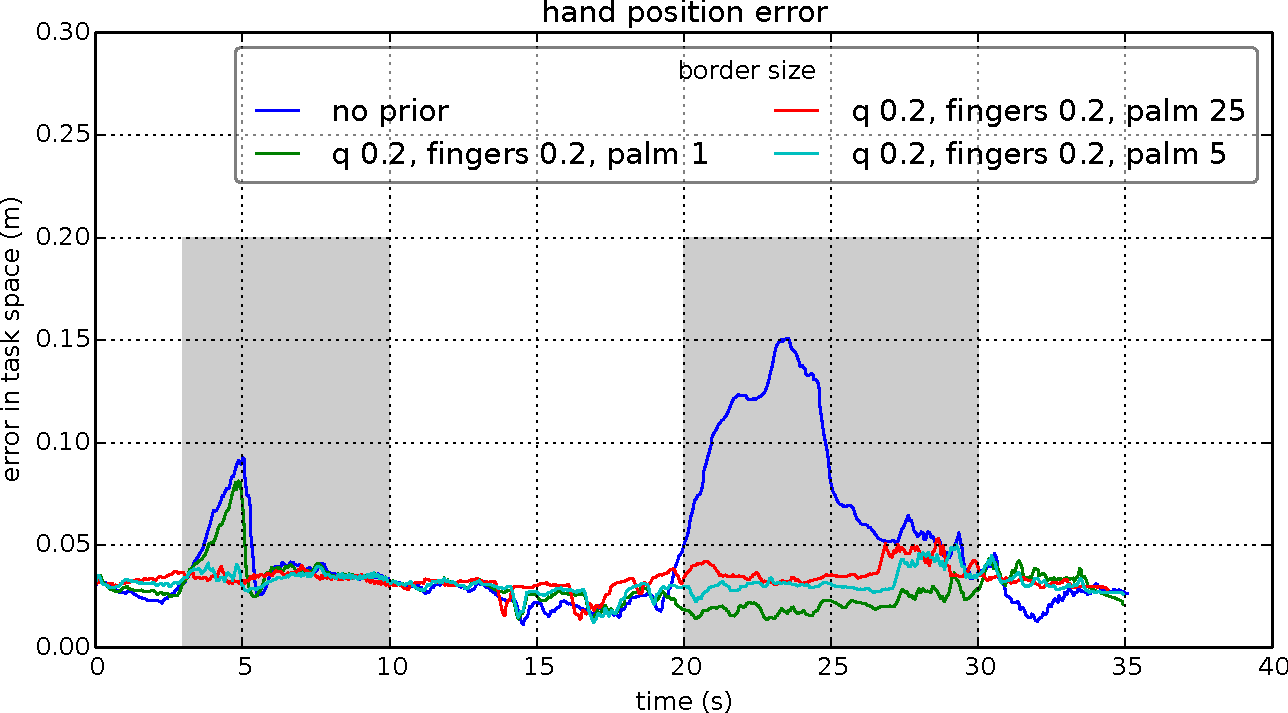
\includegraphics[width=0.5\textwidth]{images/eval_prior/inidv_weights/q0_stereo_hand_pos_error.pdf} }
%
\subfloat[orientation error]{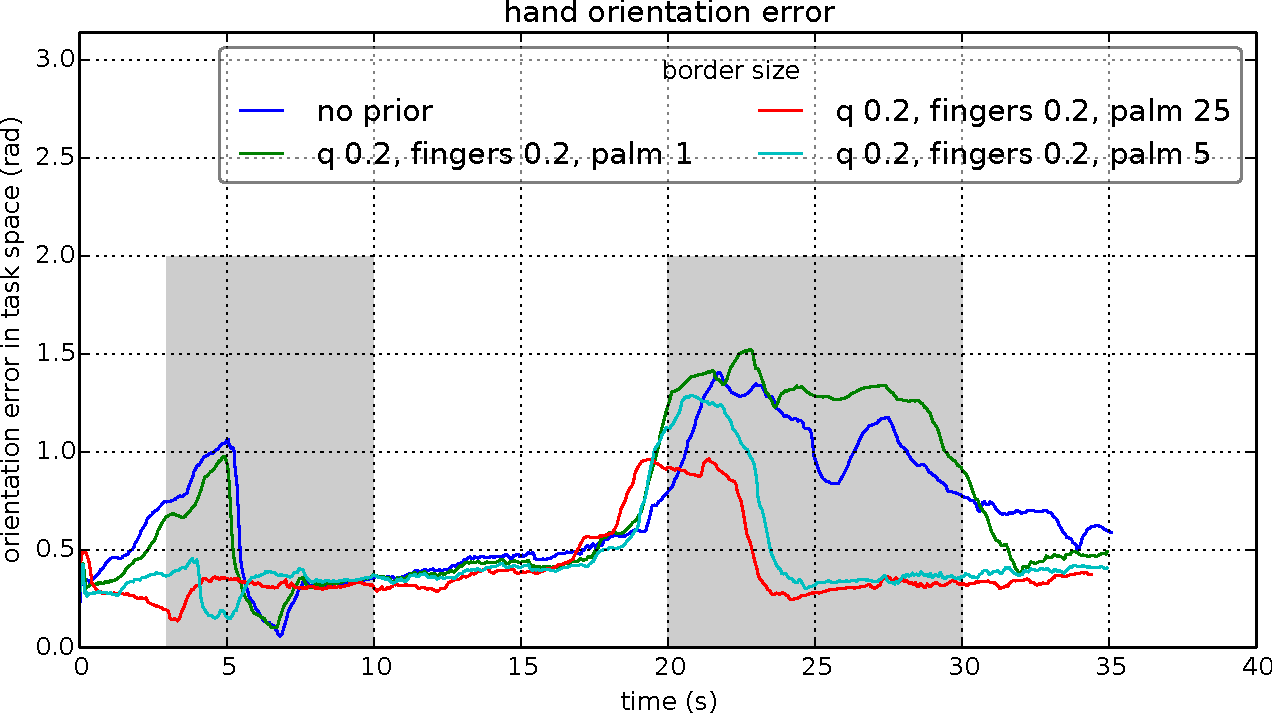
\includegraphics[width=0.5\textwidth]{images/eval_prior/inidv_weights/q0_stereo_hand_ori_error.pdf} }

\subfloat[position error]{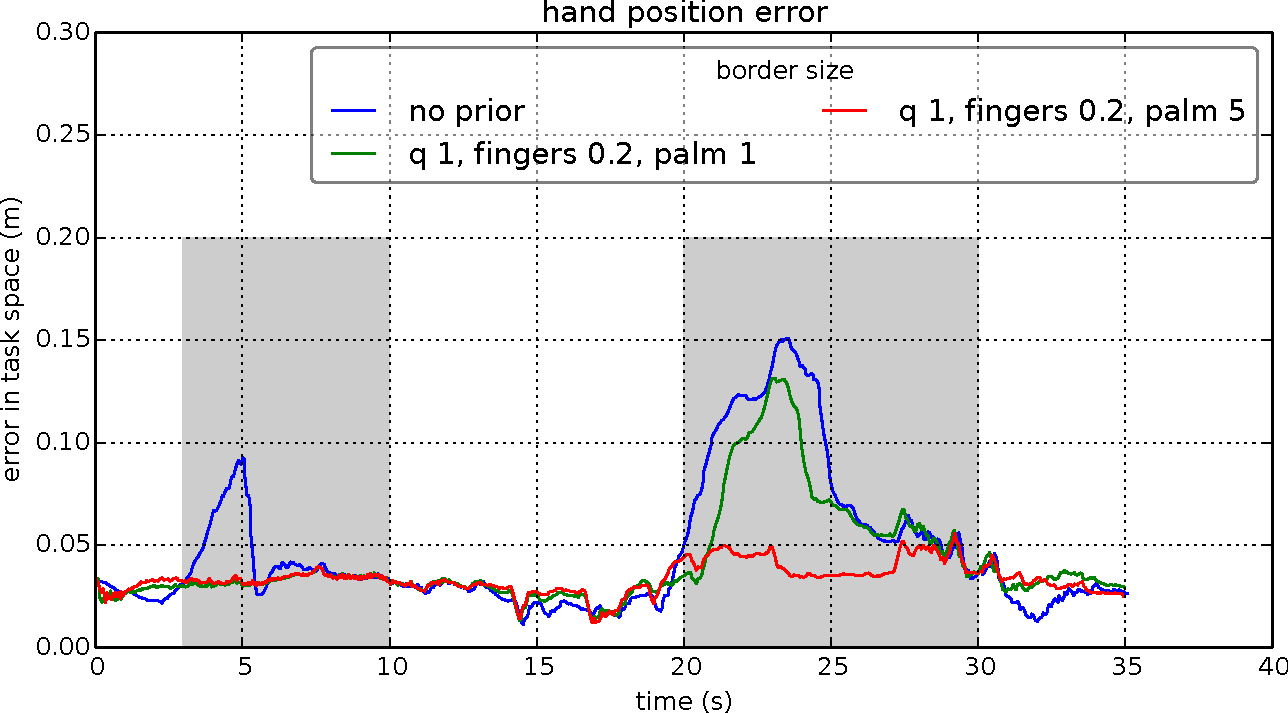
\includegraphics[width=0.5\textwidth]{images/eval_prior/inidv_weights/q1_stereo_hand_pos_error.pdf} }
%
\subfloat[orientation error]{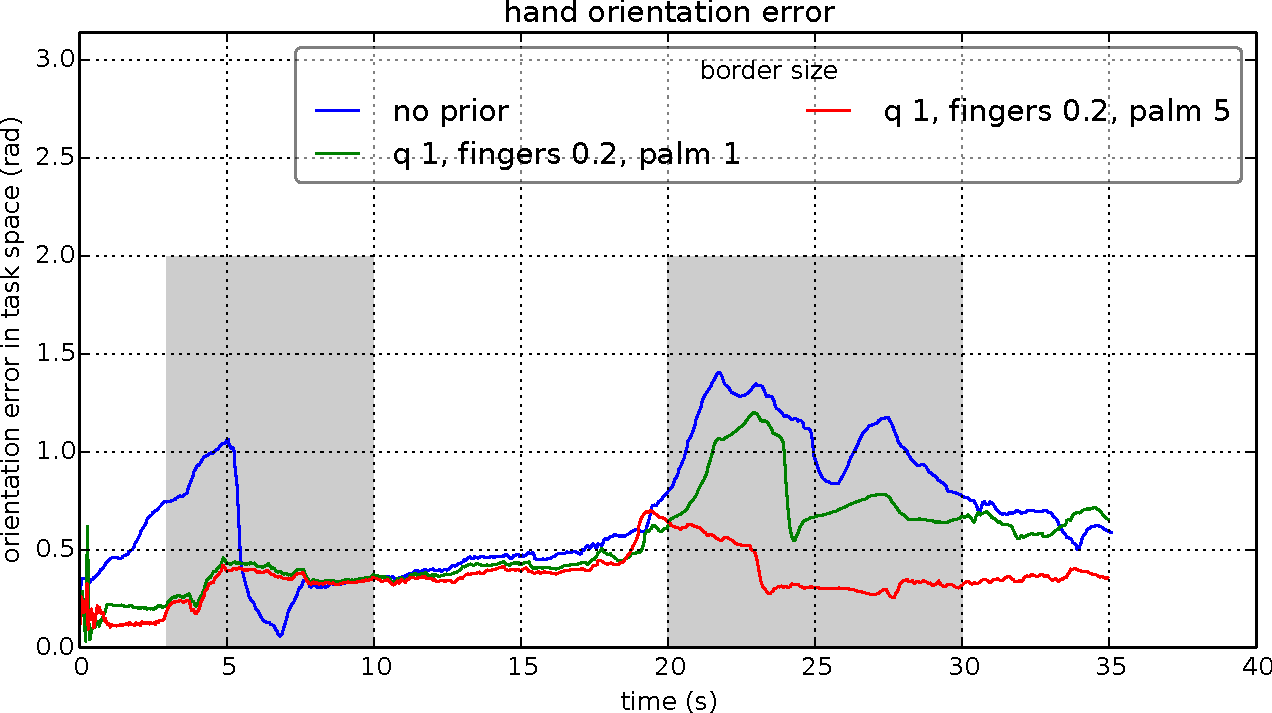
\includegraphics[width=0.5\textwidth]{images/eval_prior/inidv_weights/q1_stereo_hand_ori_error.pdf} }

\caption[Task space error for individual weighting (Exp. 1)]{Task space error for individual weighting (Exp. 1). Weights on palm joints are increased ($1$, $5$, $25$) while remaining joints are kept constant at low weights (a,b) or normal weights (c,d). The hand pose error is reduced in each case for increasing palm weights.}
\label{fig:indiv_pose_error}
\end{figure}

%\subsubsection{Object Position}
%
%Most of the time, the pose of the object (bottle) is mainly affected by the optimization. Only when there is interaction between the manipulator and the object, it gets indirectly dependant on the joint values and hence the prior weight. The object's pose is manually initialised close to the true observed state and is expected to not move until the end of the reaching phase. \Cref{fig:bottle_movement} compares the object's distance to the image origin for stereo and xtion data sets and gives an indication about its movement. The bottle in the stereo data (\cref{fig:bottle_movement_stereo}) stays, as expected, close to its initial position until the end of the reaching phase. In contrast, the bottle in the Xtion data set (\cref{fig:bottle_movement_xtion}) already moves at the beginning to its final pose.
%
%\begin{figure}[h]
%\centering
%\subfloat[stereo]{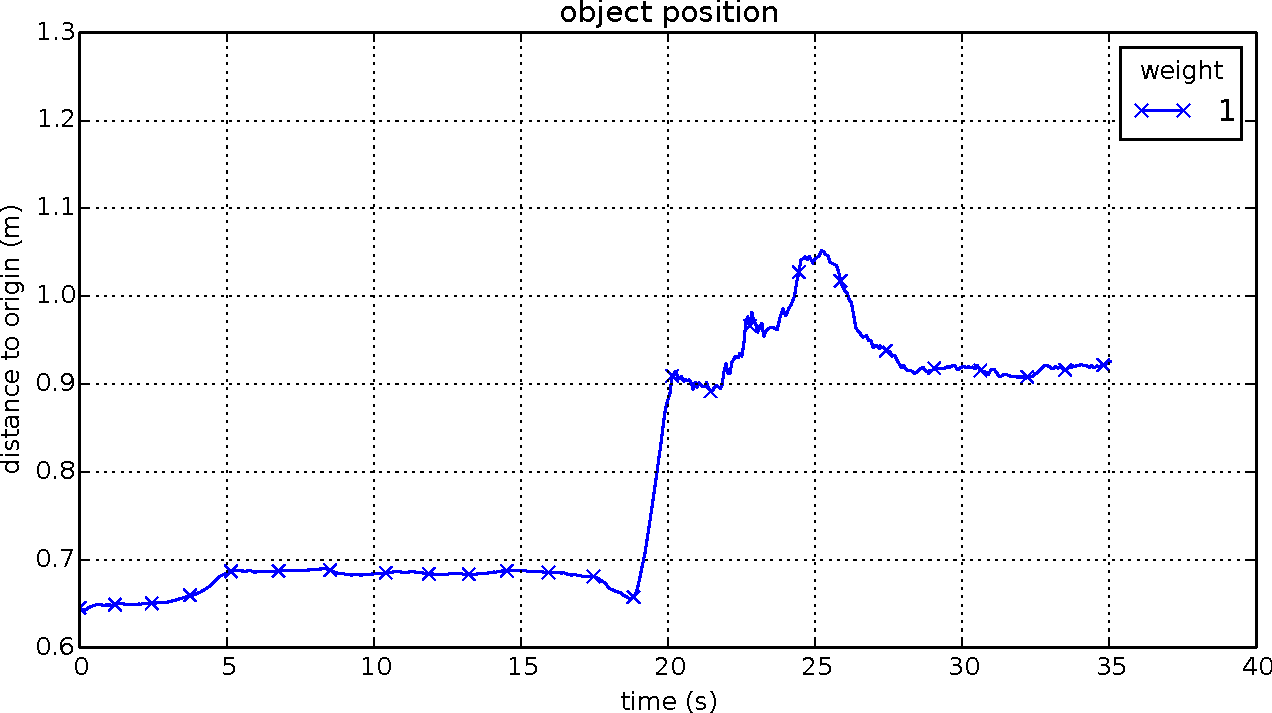
\includegraphics[width=0.5\textwidth]{images/eval_prior/stereo_obj_pos.pdf} \label{fig:bottle_movement_stereo}}
%\subfloat[xtion]{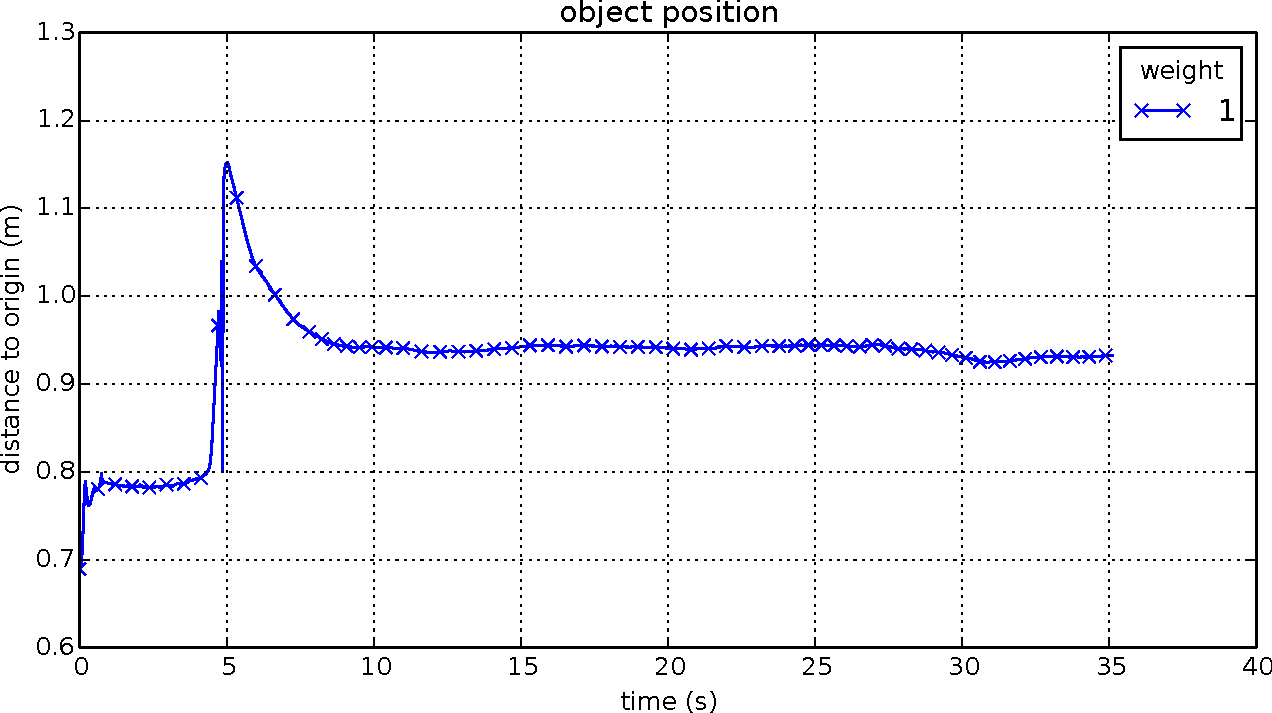
\includegraphics[width=0.5\textwidth]{images/eval_prior/xtion_obj_pos.pdf} \label{fig:bottle_movement_xtion}}
%\caption{Movement of bottle during robot arm movement}
%\label{fig:bottle_movement}
%\end{figure}
%
%Snapshots of the perceived point clouds are depicted in \cref{fig:bottle_point_cloud} for a state at the beginning of the experiment for both depth sources. A comparison of these sources show that: 1) the stereo depth source contains data with larger depth, and 2) the stereo depth source also contains more points of the object than the structured light sensor. It must be noted that the structured light sensor is mounted above the stereo sensor pointing into the same region of interest. It thus perceives the scene at a steeper angle.
%
%\begin{figure}
%\centering
%\subfloat[stereo point cloud]{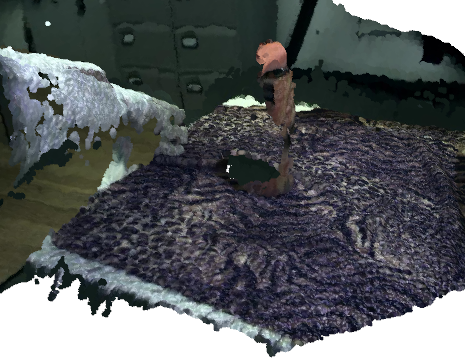
\includegraphics[width=0.4\textwidth]{images/eval_prior/stereo_bottle.png} }
%\hspace{1cm}
%\subfloat[xtion point cloud]{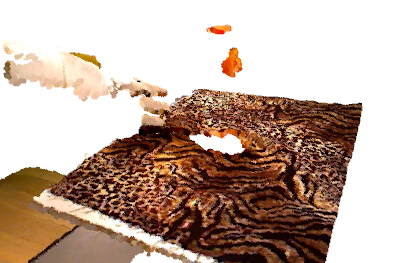
\includegraphics[width=0.4\textwidth]{images/eval_prior/xtion_bottle.png} }
%\caption{Table and bottle in stereo and xtion point cloud}
%\label{fig:bottle_point_cloud}
%\end{figure}


\subsubsection{Self-Observation Filtering using Joint Prior}

An alternative to using prior information in the optimization is to use prior information to provide the optimization with relevant data. In this sense, the reported state of the robot is used to filter its observation to only contain points close to the predicted location of the manipulator.
%In this scenario, the object is not included in tracking as relevant points cannot be obtained by self-observation.

The filtering of observed data is achieved by projecting the manipulator into the field-of-view of the robot's perception system. Each point in the disparity image that is occupied by one of the robot's projected parts is kept while all remaining values are removed. This filtered region can be further expanded on the borders of the self perceived parts. \Cref{fig:self_observation_region} demonstrates the filtered perception on stereo data for three different values for the border expansion.
%The expansion value is the size of the squared dilation kernel that is applied to the self-observation mask.

\begin{figure}[h]
\centering
\subfloat[normal mask]{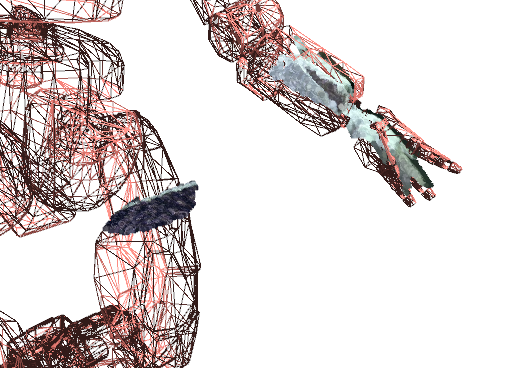
\includegraphics[width=0.3\textwidth]{images/eval_prior/filtering/filt_b0.png} }
\subfloat[expanded by 10 pxl]{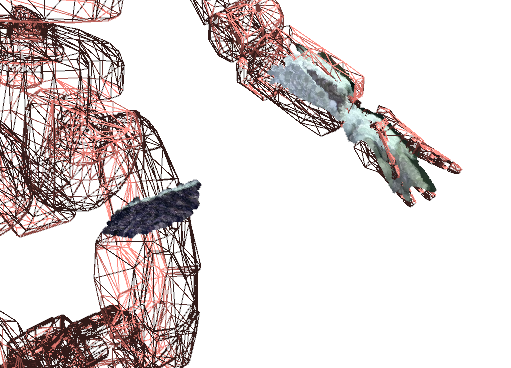
\includegraphics[width=0.3\textwidth]{images/eval_prior/filtering/filt_b10.png} }
\subfloat[expanded by 100 pxl]{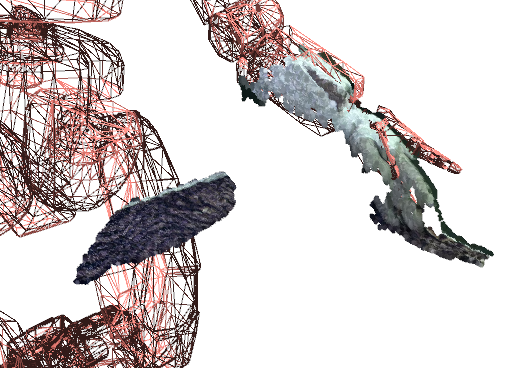
\includegraphics[width=0.3\textwidth]{images/eval_prior/filtering/filt_b100.png} }
\caption[Self-Observation filtering]{Point cloud filtering by self-observation with different expended regions.}
\label{fig:self_observation_region}
\end{figure}

In comparison to the joint position prior applied to the objective function, the joint and task space errors for self-observation filtering are given in \cref{fig:filter_joint_error,fig:filter_pose_error}. The error is again given as the deviation from the reported pose, however the joint position prior is not used in the optimization and hence, the solution is not directly driven towards the reported configuration.

As it can be easily seen for the joint space error in \cref{fig:filter_joint_error_hand,fig:filter_joint_error_arm}, there is an individual optimal value for the region expanding that minimizes the error for the finger joints (20) and the arm joints (150). While the finger joint deviation in the optimal expanded case is larger than the joint deviation using small weights (\cref{fig:stereo_joint_error_hand}), the optimal arm region expansion achieves similar results compared to the joint prior with weights around $1$ (\cref{fig:stereo_joint_error_arm}).

\begin{figure}[h]
\centering
\subfloat[finger joints]{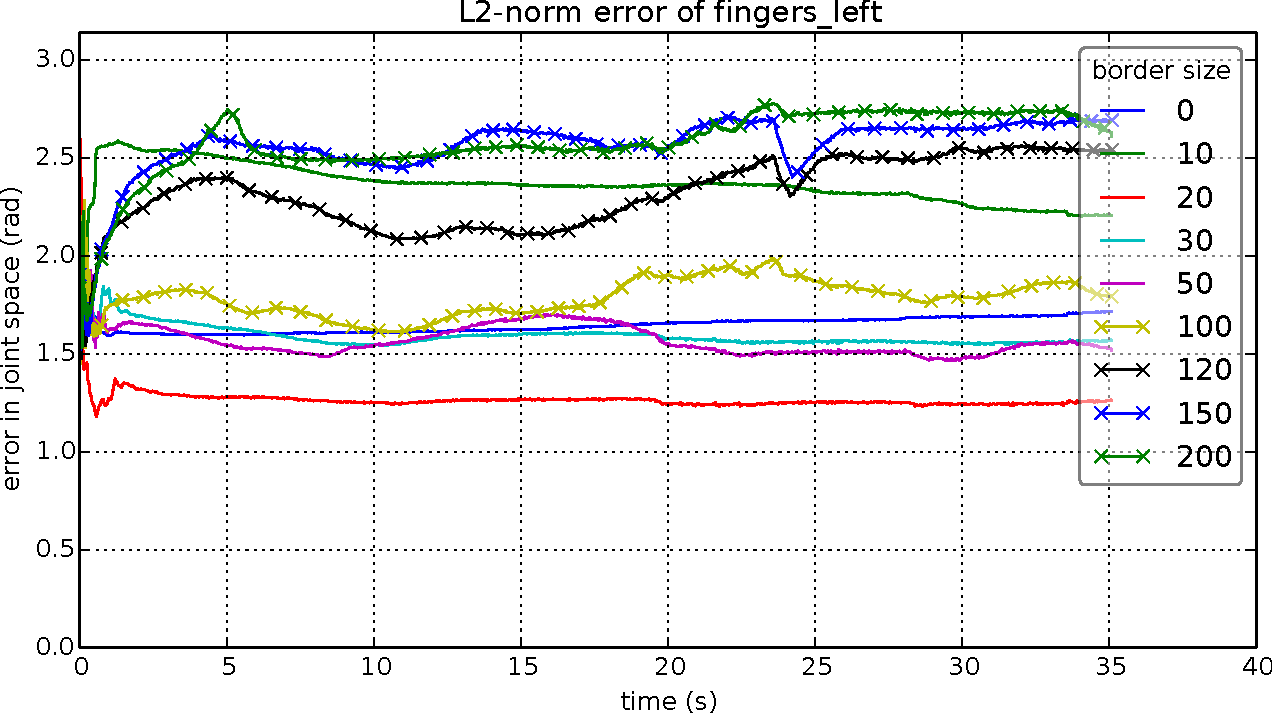
\includegraphics[width=0.5\textwidth]{images/eval_prior/filtering/stereo_finger_joint_error.pdf} \label{fig:filter_joint_error_hand}}
\subfloat[arm joints]{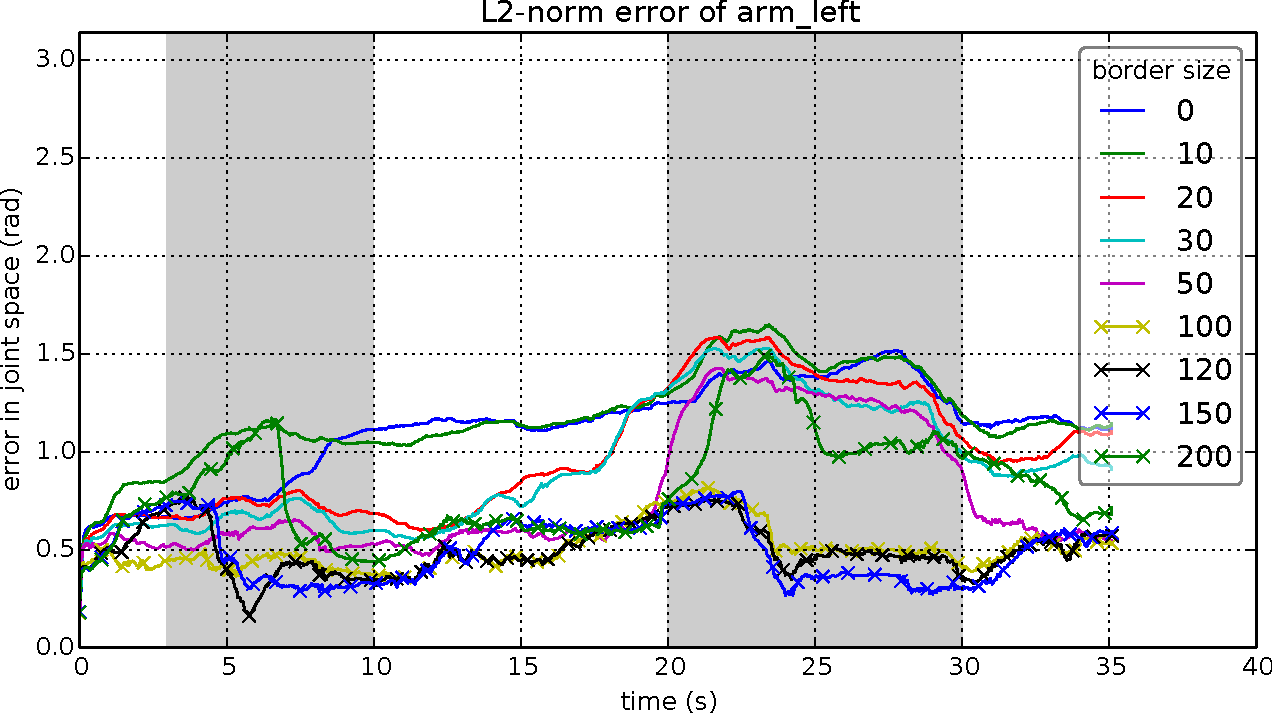
\includegraphics[width=0.5\textwidth]{images/eval_prior/filtering/stereo_arm_joint_error.pdf} \label{fig:filter_joint_error_arm}}
\caption[Joint space error for filtered perception (Exp. 1)]{Joint space error for filtered perception (Exp. 1). Individual border expansions emerge for minimizing finger joint deviation (20) and for minimizing arm joint deviation (150).}
\label{fig:filter_joint_error}
\end{figure}

For large expansions of the self-observation mask (200), the hand position error in \cref{fig:filter_hand_pos_error} behaves similar to the case where no prior is used on the unfiltered observation (\cref{fig:stereo_hand_pos_error}). Further, in phases of contact with surrounding objects a smaller region expansion is preferable over larger borders. The reason for this is that large self-observation masks will include nearby objects, which again will distract the optimization without prior. A larger region expansion is preferable in phases where the manipulator is moving in free space (time between highlighted phases).
The hand orientation error behaves similar to the arm joint error, in particular an optimal region expansion (150) emerges and larger region expansions are favourable in general.

\begin{figure}
\centering
\subfloat[position error]{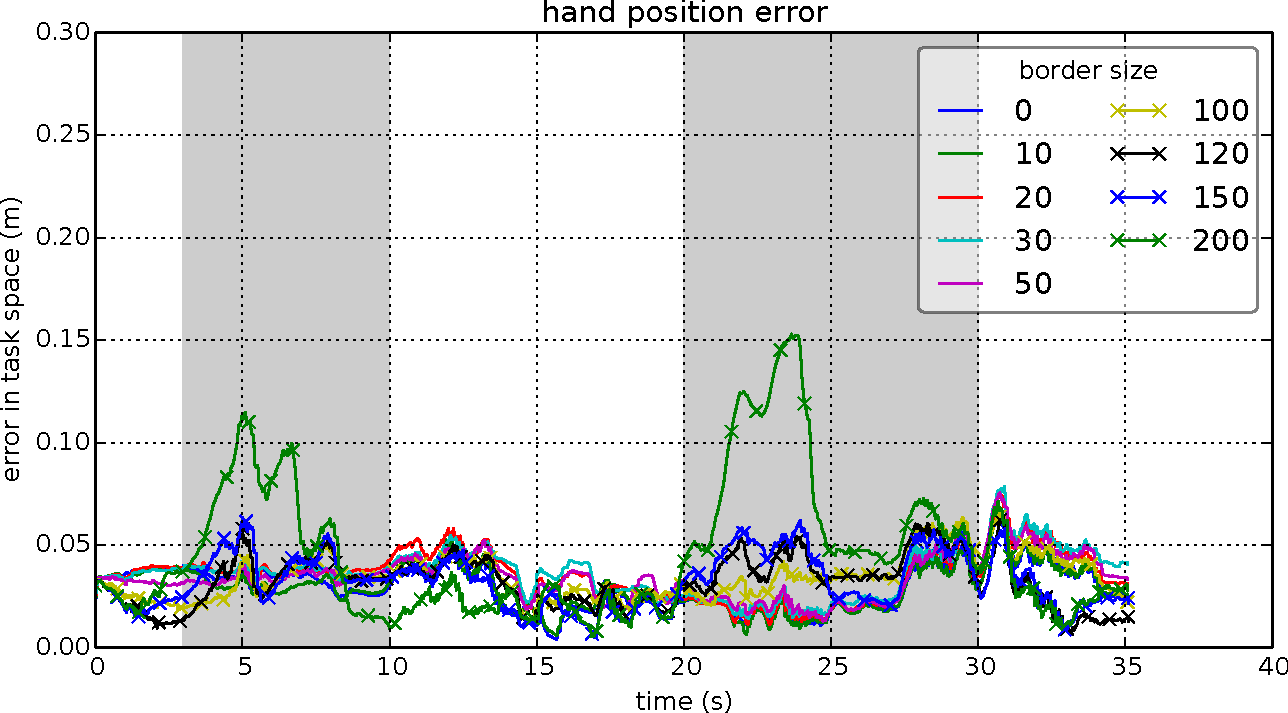
\includegraphics[width=0.5\textwidth]{images/eval_prior/filtering/stereo_hand_pos_error.pdf} \label{fig:filter_hand_pos_error}}
\subfloat[orientation error]{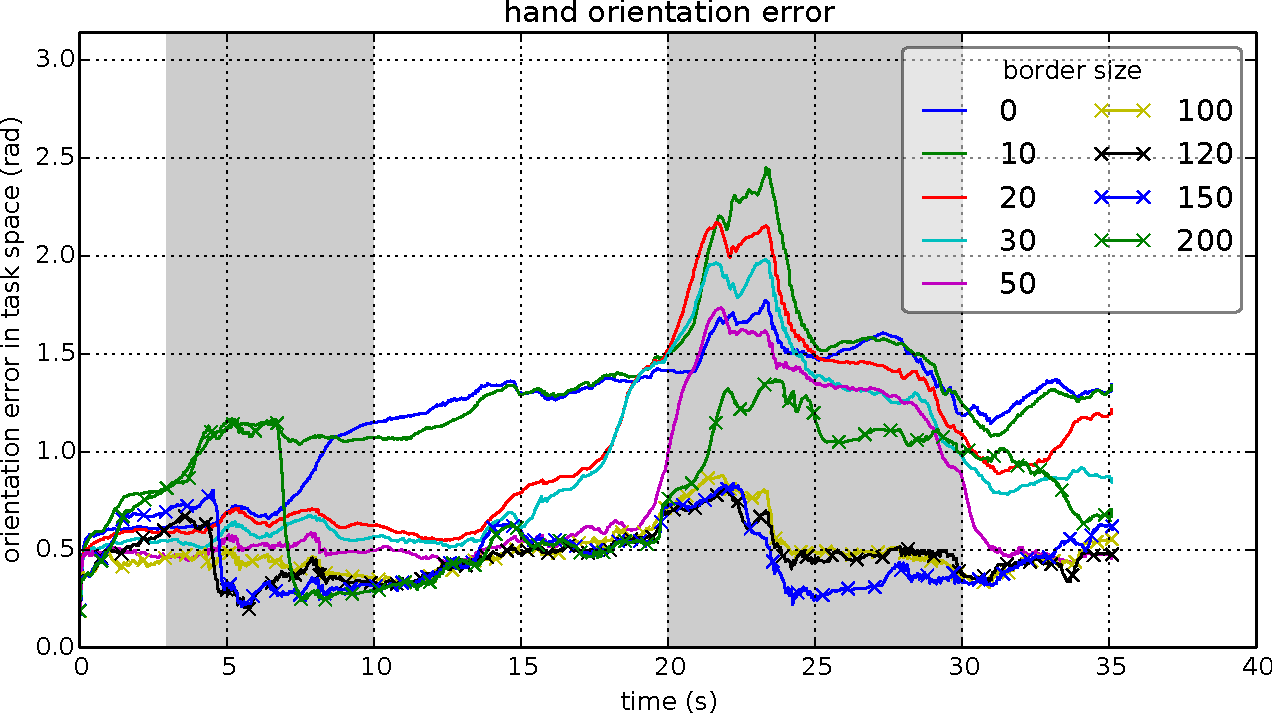
\includegraphics[width=0.5\textwidth]{images/eval_prior/filtering/stereo_hand_ori_error.pdf} \label{fig:filter_hand_ori_error}}
\caption[Task space error for filtered perception (Exp. 1)]{Task space error for filtered perception (Exp. 1). Smaller border expansions are preferable over large borders in phases where the manipulator is close to objects (highlighted).}
\label{fig:filter_pose_error}
\end{figure}


\subsection{Interpretation}

With the signed distance as the only objective function, the optimization is driven away from the reported state, with which it is initialized, whenever nearby but unrelated depth data is assigned to the robot model. Hence we conclude that \cref{hyp:distracting_readings} is true. By augmenting the objective function with an objective related to the reported state as the reference, this effect can be reduced.

Across all weighting schemes and depth sources, we can see that weighting in respect to the deviation from the reported pose: (1) reduces the deviation of finger joint positions over the whole sequence of the trials by already choosing a small prior weight, (2) contributes most in movement phases that follow states where the manipulator is in contact with the scene (table, object). The application of individual weighting of joint deviations showed that by selecting specific joints, the task space error can be reduced while keeping the flexibility of preferring other objectives for the remaining parts of the robot model. For both assessed weighting schemes, it turned out that weights need to be chosen carefully to prevent overshooting on the reported state and hence the oscillation of the estimate state. Neglecting the issue of oscillating around the optimum, \cref{hyp:prior_information} is also considered to be verified.

The self-observation filtering of the perception showed that using prior information to shape the input to the optimization also counteracts the issue of distracting observation. By using prior information to filter relevant data, the reported robot state only indirectly improves the optimization result.
The decoupling of the optimization from the reported joint values prevents cases of overfitting on the reported state by limiting the bias from prior information.

The assessed prior information is by design only applicable to the robot model. The tracked object remains to be driven by the signed distance function and hence relies on relevant depth data assigned to the object model.
%We saw that this is an issue for observing from an low angle to the object's principal axes.


\section{Experiment 2: Ground Truth Comparison}
\label{sec:hand_pose_error}

An experiment was conducted that contains depth data measurements from the manipulator alone, without distracting depth readings nearby. As in the previous experiment, forward kinematics on the reported and estimated joint configuration was used to obtain the pose of the manipulator in task space. Additionally, the Vicon system introduced earlier provides ground truth data of the hand palm pose.


\subsection{Hypotheses}

The experiment has been designed to (1) apply the tracking of the manipulator in a scene without distractions, and (2) to compare the reported and estimated robot configuration with the ground truth poses reported by the Vicon tracking system.

Without distracting sensor readings, we expect that the use of the joint position prior will not have a strong impact on the deviation from the reported robot configuration. If the manipulator is fully observed in the depth data, tracking the manipulator should result in a hand pose close to the true hand pose which itself should coincide with the reported hand pose.

\begin{hypothesis}(No effect of joint position prior)\\
There is no significant effect of applying a joint position prior on observations containing solely the manipulator.
\label{hyp:no_prior_effect}
\end{hypothesis}

\begin{hypothesis}(Matching hand pose)\\
Reported and estimated left hand poses agree with the measured hand pose.
\label{hyp:matching_hand_pose}
\end{hypothesis}


\subsection{Setup}

The robot is placed in a nominal position and its manipulator moves from this state into the field of view of the camera (\cref{fig:vicon_free_movement}). To observe the manipulator and its fingers from different perspectives, the hand and the fingers are actuated by a certain degree. The data set is therefore divided into two parts: \textit{arm movement} (experiment 2a), where mainly the shoulder and the forearm joints are actuated, and \textit{finger movement} (experiment 2b) where all fingers are actuated at the same time. During the complete experiment, Vicon markers are attached to the pelvis and backside of the palm to track the orientation of both robot frames (\cref{fig:vicon_marker}).

\begin{figure}[h]
\captionsetup{width=0.45\textwidth}
\centering
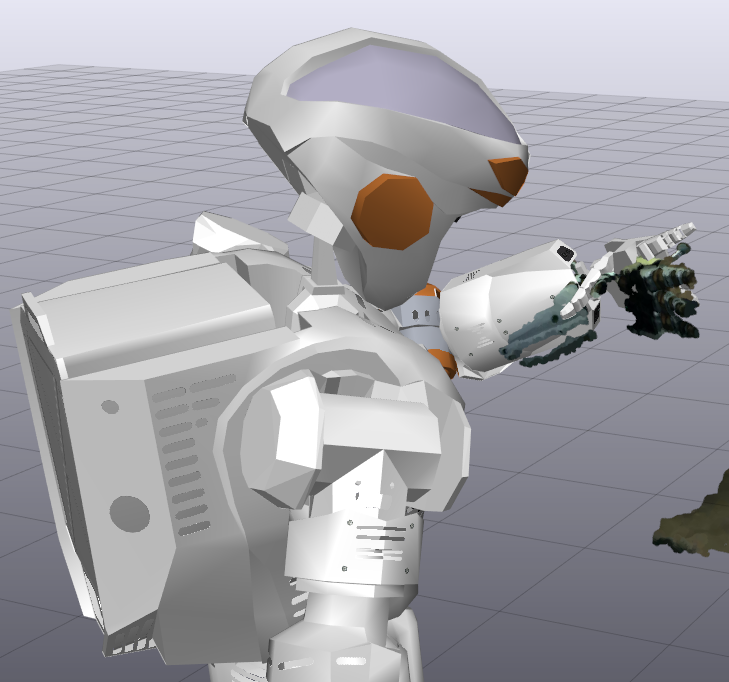
\includegraphics[width=0.4\textwidth]{images/eval_vicon/sequence/setting.png}
\caption[Experiment 2: Setup]{Experiment 2: Setup in which a robot is observing its own manipulator.}
\label{fig:vicon_free_movement}
\end{figure}

\paragraph{Experiment 2a:}
The \textit{arm movement} sequence contains three movement phases (\cref{tab:vic_arm_movement_phases}) of which 3 final states are depicted in \cref{fig:arm_movement_states}.

\begin{table}[h]
\centering
\begin{tabular}{|c|l|l|}
\hline
 & \emph{time (s)} & \emph{movement description} \\
\hline
1 & 0$\dots$50 & no movement, hand in lower camera view \\
\hline
2 & 50$\dots$54 & arm movement up \\
\hline
3 & 85$\dots$90 & hand palm turning up (forearm joint) \\
\hline
4 & 125$\dots$130 & hand palm turning down (forearm joint) \\
\hline
\end{tabular}
\caption{Phases of arm movement (Exp. 2a)}
\label{tab:vic_arm_movement_phases}
\end{table}

\newlength{\imgwidth}
\setlength{\imgwidth}{0.26\textwidth}

\begin{figure}
\centering
\begin{tabular}{cc:c:c}
& \textit{Phase 2 (t=55\si{\second})} & \textit{Phase 3 (t=91\si{\second})} & \textit{Phase 4 (t=132\si{\second})} \\
& (facing towards robot) & (facing up) & (facing down)\\
\rotatebox{90}{ \hspace{0.45cm} camera image } & 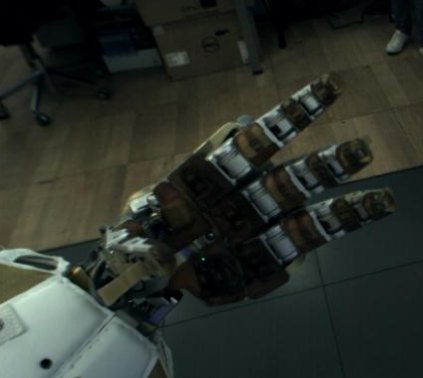
\includegraphics[width=\imgwidth]{images/eval_vicon/sequence/arm_movement/arm_movement_cam_view55.png} & 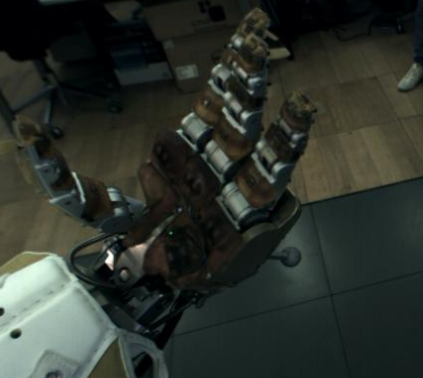
\includegraphics[width=\imgwidth]{images/eval_vicon/sequence/arm_movement/arm_movement_cam_view91.png} & 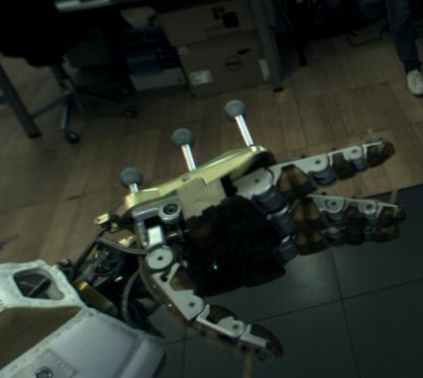
\includegraphics[width=\imgwidth]{images/eval_vicon/sequence/arm_movement/arm_movement_cam_view132.png} \\
\rotatebox{90}{ \hspace{1cm} point cloud } & 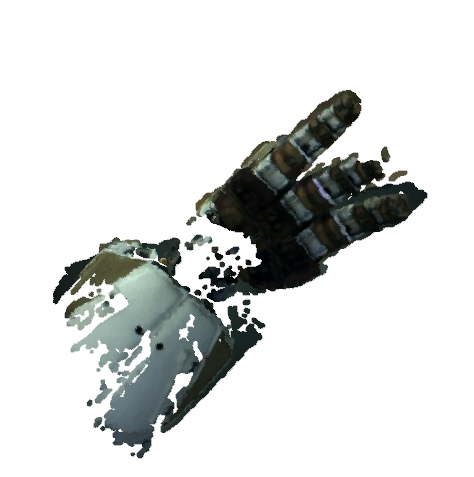
\includegraphics[width=\imgwidth]{images/eval_vicon/sequence/arm_movement/obs_55.png} & 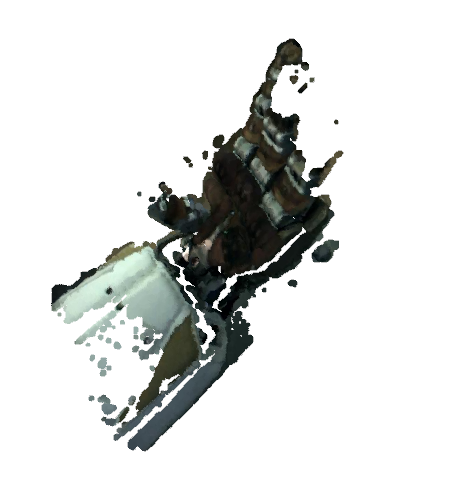
\includegraphics[width=\imgwidth]{images/eval_vicon/sequence/arm_movement/obs_91.png} & 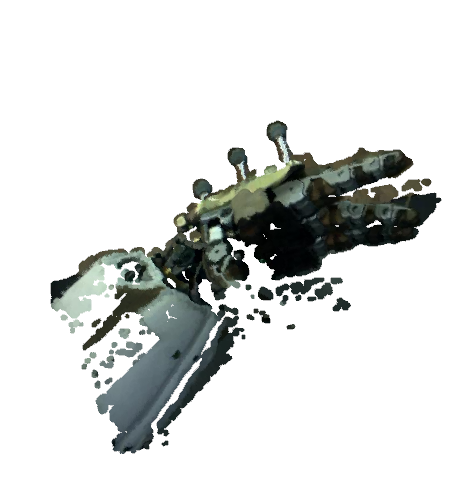
\includegraphics[width=\imgwidth]{images/eval_vicon/sequence/arm_movement/obs_132.png} \\
\rotatebox{90}{ \hspace{1cm} reported state } & 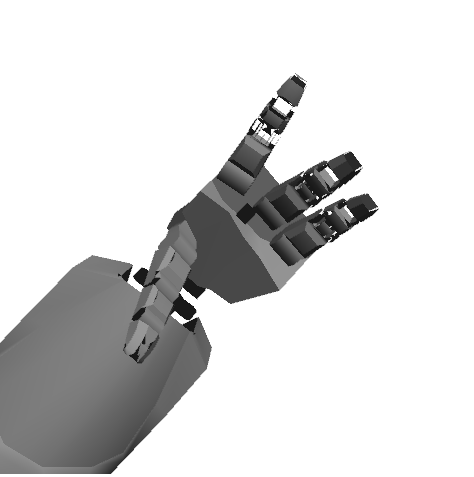
\includegraphics[width=\imgwidth]{images/eval_vicon/sequence/arm_movement/rep_55.png} & 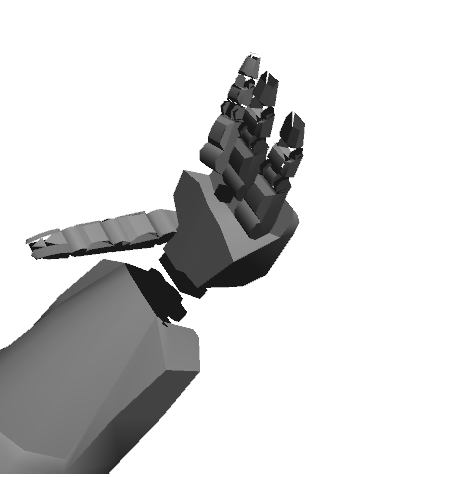
\includegraphics[width=\imgwidth]{images/eval_vicon/sequence/arm_movement/rep_91.png} & 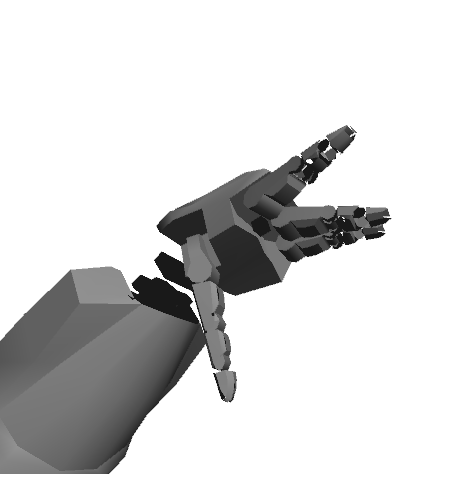
\includegraphics[width=\imgwidth]{images/eval_vicon/sequence/arm_movement/rep_132.png} \\
\end{tabular}
\caption[Arm movement sequence]{Experiment 2a (\textit{arm movement}): Sequence of states in which the manipulator is observed from different viewing angles. \textit{Upper row:} camera image, \textit{Middle row:} point cloud observation, \textit{Lower row:} reported state.}
\label{fig:arm_movement_states}
\end{figure}

\FloatBarrier

\paragraph{Experiment 2b:}
The \textit{finger movement} sequence contains 7 movement phases in total (\cref{tab:vic_finger_movement_phases}) of which 6 states are depicted in \cref{fig:finger_movement_states}.

\begin{table}[h]
\centering
\begin{tabular}{|c|l|l|}
\hline
 & \emph{time (s)} & \emph{movement description} \\
\hline
1 & 0$\dots$30 & no movement, palm facing towards camera \\
\hline
2 & 30$\dots$33 & fingers closing 25\% \\
\hline
3 & 56$\dots$59 & fingers closing 50\% \\
\hline
4 & 72$\dots$75 & fingers opening \\
\hline
5 & 100$\dots$104 & hand palm turning up (forearm joint) \\
\hline
6 & 127$\dots$130 & fingers closing 25\% \\
\hline
7 & 147$\dots$150 & fingers closing 50\% \\
\hline
8 & 156$\dots$159 & fingers opening \\
\hline
\end{tabular}
\caption{Phases of finger movement (Exp. 2b)}
\label{tab:vic_finger_movement_phases}
\end{table}

%\newlength{\imgwidth}
\setlength{\imgwidth}{0.26\textwidth}

\begin{figure}
\centering
\begin{tabular}{cc:c:c}
\hline
& \textit{Phase 1 (t=19\si{\second})} & \textit{Phase 2 (t=33\si{\second})} & \textit{Phase 3 (t=61\si{\second})}\\
& (opened) & (closed $\sim 25\%$) & (closed $\sim 50\%$)\\

\rotatebox{90}{ \hspace{0.25cm} camera image } & 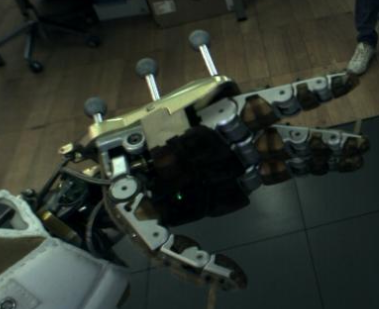
\includegraphics[width=\imgwidth]{images/eval_vicon/sequence/finger_movement/finger_movement_cam_view19.png} & \includegraphics[width=\imgwidth]{images/eval_vicon/sequence/finger_movement/finger_movement_cam_view33.png} & \includegraphics[width=\imgwidth]{images/eval_vicon/sequence/finger_movement/finger_movement_cam_view61.png} \\

\rotatebox{90}{ \hspace{0.25cm} point cloud } & \includegraphics[width=\imgwidth]{images/eval_vicon/sequence/finger_movement/obs_0.png} & \includegraphics[width=\imgwidth]{images/eval_vicon/sequence/finger_movement/obs_33.png} & \includegraphics[width=\imgwidth]{images/eval_vicon/sequence/finger_movement/obs_61.png} \\

\rotatebox{90}{ \hspace{0.25cm} reported state } & \includegraphics[width=\imgwidth]{images/eval_vicon/sequence/finger_movement/rep_0.png} & \includegraphics[width=\imgwidth]{images/eval_vicon/sequence/finger_movement/rep_33.png} & \includegraphics[width=\imgwidth]{images/eval_vicon/sequence/finger_movement/rep_61.png} \\
\hline
& \textit{Phase 5 (t=105\si{\second})} & \textit{Phase 6 (t=133\si{\second})} & \textit{Phase 7 (t=152\si{\second})}\\
& (opened) & (closed $\sim 25\%$) & (closed $\sim 50\%$)\\

\rotatebox{90}{ \hspace{0.25cm} camera image } & \includegraphics[width=\imgwidth]{images/eval_vicon/sequence/finger_movement/finger_movement_cam_view105.png} & \includegraphics[width=\imgwidth]{images/eval_vicon/sequence/finger_movement/finger_movement_cam_view133.png} & \includegraphics[width=\imgwidth]{images/eval_vicon/sequence/finger_movement/finger_movement_cam_view152.png} \\

\rotatebox{90}{ \hspace{0.25cm} point cloud } & \includegraphics[width=\imgwidth]{images/eval_vicon/sequence/finger_movement/obs_105.png} & \includegraphics[width=\imgwidth]{images/eval_vicon/sequence/finger_movement/obs_133.png} & \includegraphics[width=\imgwidth]{images/eval_vicon/sequence/finger_movement/obs_152.png} \\

\rotatebox{90}{ \hspace{0.25cm} reported state } & \includegraphics[width=\imgwidth]{images/eval_vicon/sequence/finger_movement/rep_105.png} & \includegraphics[width=\imgwidth]{images/eval_vicon/sequence/finger_movement/rep_133.png} & \includegraphics[width=\imgwidth]{images/eval_vicon/sequence/finger_movement/rep_152.png} \\
\end{tabular}
\caption[Finger movement sequence]{Experiment 2b (\textit{finger movement}): Sequence of states in which the fingers are close to certain degree (order from left to right: open, closed $\sim 25\%$, closed $\sim 50\%$). \textit{Upper sequence:} Hand palm facing down, \textit{Lower sequence:} Hand palm facing towards robot. In each sequence: \textit{Upper row:} camera image, \textit{Middle row:} point cloud observation, \textit{Lower row:} reported state.}
\label{fig:finger_movement_states}
\end{figure}

Both data sets show that due to self-occlusion, the manipulator cannot be fully observed within a single observation. In states where the palm is facing down, the Vicon marker can be observed in the point cloud data.

%\FloatBarrier


\subsection{Results}

The shown errors are the L2 norm of the joint and task space errors as defined in \cref{sec:prior_results}. The common weighting scheme \emph{Weighted L2 norm of joint position deviation} (objective function \cref{eqn:objf_weightedL2}) is applied for the joint position prior when comparing different weights. Time and durations are given in seconds.

\subsubsection{Joint Space Error}

The joint space error for both sequences is shown separately for finger and arm joints in \cref{fig:am_joint_error,fig:fm_joint_error}. It can be noticed that increasing prior weights reduces the joint position deviation in the case of less distracting observations. However, the effect is not as significant as it is for observations with distractions due to close solutions after proper initialisation.

\begin{figure}[h]
\centering
\subfloat[finger joints]{\includegraphics[width=0.5\textwidth]{images/eval_vicon/val_arm_joint_error_fingers.pdf} }
\subfloat[arm joints]{\includegraphics[width=0.5\textwidth]{images/eval_vicon/val_arm_joint_error_arm.pdf} }
\caption{Experiment 2a: joint space error}
\label{fig:am_joint_error}
\end{figure}

\begin{figure}[h]
\centering
\subfloat[finger joints]{\includegraphics[width=0.5\textwidth]{images/eval_vicon/val_finger_joint_error_fingers.pdf} }
\subfloat[arm joints]{\includegraphics[width=0.5\textwidth]{images/eval_vicon/val_finger_joint_error_arm.pdf} }
\caption{Experiment 2b: joint space error}
\label{fig:fm_joint_error}
\end{figure}

In states where the palm is facing towards the camera and large continuous hand parts can be observed, the tracked configuration of the arm is already so close to the reported configuration, that an additional joint position prior has no effect. This is the case after phase 2 for the \textit{arm movement} data set ($55\leq t \leq84$) and phase 5 for the \textit{finger movement} data set ($t \geq 105$).


\subsubsection{Task Space Error}

To evaluate the task space error, we compare the reported and the estimated hand pose with the hand pose measured by the Vicon tracking system. The shown errors are the L2 norm of the 3D pose and 3D rotation difference from Vicon pose to the reported and estimated pose.

The error plots in \cref{fig:vic_error_arm_movement,fig:vic_error_finger_movement} compare the effect of prior weighting on the estimated configurations against the reported configuration (which is not effected by the prior). Comparison plots for the task space error on the reported and on the estimated pose without prior are shown separately for a clearer distinction.

\begin{figure}[h]
\centering
\subfloat[position error]{\includegraphics[width=0.5\textwidth]{images/eval_vicon/val_arm_pos_error.pdf} }
\subfloat[orientation error]{\includegraphics[width=0.5\textwidth]{images/eval_vicon/val_arm_ori_error.pdf} }

\subfloat[position error (no prior)]{\includegraphics[width=0.5\textwidth]{images/eval_vicon/val_arm_pos_error_nop.pdf} }
\subfloat[orientation error (no prior)]{\includegraphics[width=0.5\textwidth]{images/eval_vicon/val_arm_ori_error_nop.pdf} }

\caption[Arm movement, hand pose error]{Experiment 2a: Hand pose error of the reported and estimated robot state compared to the Vicon hand marker pose.}
\label{fig:vic_error_arm_movement}
\end{figure}

The following general statements can be made: (1) neither the reported nor the estimated hand poses agree with the Vicon hand pose, (2) the reported hand pose is closer to the Vicon hand pose than the estimated hand pose for most of the duration.

From both data sets it can be noticed that the estimated pose is closer to the Vicon pose in the same states where the joint deviation from the reported configuration is small. In particular the orientation error drops significantly in these states where large portions of the palm are observable (\textit{arm movement}: $55\leq t \leq84$, \textit{finger movement}: $t \geq 105$). In contrast, the error increases when the manipulator is observed from the side, e.g. when fingers are occluding each other (\textit{arm movement}: $t \geq 132$, \textit{finger movement}: $t \leq 104$).

\begin{figure}[h]
\centering
\subfloat[position error]{\includegraphics[width=0.5\textwidth]{images/eval_vicon/val_finger_pos_error.pdf} }
\subfloat[orientation error]{\includegraphics[width=0.5\textwidth]{images/eval_vicon/val_finger_ori_error.pdf} }

\subfloat[position error (no prior)]{\includegraphics[width=0.5\textwidth]{images/eval_vicon/val_finger_pos_error_nop.pdf} }
\subfloat[orientation error (no prior)]{\includegraphics[width=0.5\textwidth]{images/eval_vicon/val_finger_ori_error_nop.pdf} }

\caption[Finger movement, hand pose error]{Experiment 2b: Hand pose error of the reported and estimated robot state compared to the Vicon hand marker pose.}
\label{fig:vic_error_finger_movement}
\end{figure}


\subsection{Interpretation}

Tracking with manipulator-only observed data showed that there is still an effect of using prior information. However, this effect is not as significant as in distracting scenes and it is minimal in states where large portions of the manipulator can be observed from a single observation. The performance of the tracking and hence the effect of prior information is view dependent. Prior information is still useful for inconclusive observations, e.g. self-occlusion. Despite this, \cref{hyp:no_prior_effect} is considered as true.

The observation of the Vicon marker in the depth data of the manipulator, e.g. when the hand palm is facing down, is not examined in this evaluation. These markers are required to obtain the ground truth data but they certainly provide  readings that could distract the optimization.

An interesting result from this evaluation is that neither the reported nor the estimated hand pose agree with the Vicon hand pose. The measured discrepancy of reported position and Vicon marker position is at least \SI{1.5}{\cm}. Using a strong prior in such scenario thus can only provide an optimal solution to some extent, e.g. as long as the reported configuration is closer to the true configuration than the estimate. \Cref{hyp:matching_hand_pose} is considered as not verified and needs further investigation.


\section{Joint Calibration}

The data set collected in the previous experiment in \cref{sec:hand_pose_error} will be used to investigate the issue of mismatching hand poses of the reported and estimated state from the Vicon hand pose that is considered as ground truth.

\subsection{Hypothesis}

Under the assumption that the tracking obtains the true robot configuration, that is the estimated hand pose agrees with the Vicon hand pose, the joint position discrepancy (1) from reported configuration to configuration at Vicon pose, and (2) from reported configuration to estimated configuration, should be similar.

\begin{hypothesis}(Matching joint offset)\\
The individual joint position deviations from reported configuration to Vicon configuration and to estimated configuration are similar.
\label{hyp:matching_joint_offset}
\end{hypothesis}

\subsection{Results}

The individual arm joint position offsets for the arm movement and finger movement data sets (\cref{fig:estimated_offsets}) show that the discrepancy of estimated to reported joints position is not constant over time. Considering that the hand is directly connected to the forearm by two joints (\texttt{leftWristRoll/Pitch}), it is interesting to notice that \texttt{leftWristPitch} does not have a discrepancy to the reported joint position value, whereas \texttt{leftWristRoll} changes significantly over time.

\Cref{tab:avg_offsets_comparison} summarizes the offsets for the estimated (\textit{dart}, averaged over time) and reported (\textit{vicon}, optimized on pose) joint position offsets. As the manipulator tracking considers the kinematic chain from image centre to palm and the Vicon marker pose gives the final transformation for the kinematic chain from pelvis to palm, the arm joints are the common joints whose offsets are considered for comparison.
The correlation between the averaged \textit{dart} offsets and \textit{vicon} offsets are given as $0.3366$ for the arm data set and $0.1054$ for the finger data set.

\begin{figure}[h]
\centering
\subfloat[Arm movement (experiment 2a)]{\includegraphics[width=0.5\textwidth]{images/offset/dart_arm_offset.pdf} }
\subfloat[Finger movement (experiment 2b)]{\includegraphics[width=0.5\textwidth]{images/offset/dart_finger_offset.pdf} }

\caption[Estimated offsets]{Individual offsets of reported joint configuration to DART's estimated joint configuration}
\label{fig:estimated_offsets}
\end{figure}


\begin{table}[h]
\centering
% table with aligned decimal points
\begin{tabular}{|l||S[table-format=2.5]|S[table-format=2.5]||S[table-format=2.5]|S[table-format=2.5]||>{\columncolor[gray]{0.9}}S[table-format=2.8]|}
\hline
 & \multicolumn{5}{c|}{joint positions offsets} \\
\hline
 & \multicolumn{2}{c||}{arm data set (Exp. 2a)} & \multicolumn{2}{c||}{finger data set (Exp. 2b)} &  \multicolumn{1}{c|}{complete} \\
\hline
\multicolumn{1}{|c||}{\textit{joint name}} & \textit{dart} & \textit{vicon} & \textit{dart} & \textit{vicon} & \multicolumn{1}{c|}{\textit{vicon}} \\
\hline
\hline
\texttt{torsoYaw} &  & 0.00059 &  & -0.00118 & 0.01319969 \\
\hline
\texttt{torsoPitch} &  & 0.01166 &  & 0.00554 & 0.01062786 \\
\hline
\texttt{torsoRoll} &  & 0.00510 &  & 0.00195 & -0.00483674 \\
\hline
\texttt{leftShoulderPitch} & -0.05627 & 0.01258 & -0.01713 & 0.02658 & 0.00461001 \\
\hline
\texttt{leftShoulderRoll} & -0.12866 & 0.00288 & -0.11559 & -0.01822 & -0.0095907 \\
\hline
\texttt{leftShoulderYaw} & -0.00503 & 0.01045 & -0.09895 & -0.01157 & 0.03021091 \\
\hline
\texttt{leftElbowPitch} & 0.14880 & 0.00818 & 0.08986 & 0.02588 & 0.00446155 \\
\hline
\texttt{leftForearmYaw} & -0.16338 & 0.00166 & -0.08339 & 0.01627 & 0.00580287 \\
\hline
\texttt{leftWristRoll} & -0.18549 & 0.01169 & -0.35942 & 0.01820 & 0.02037348 \\
\hline
\texttt{leftWristPitch} & 0.00620 & 0.01953 & 0.00195 & -0.00389 & 0.02790135 \\
\hline
\end{tabular}
\caption[Joint position offsets]{Joint position offset for kinematic chain \textit{pelvis} to \textit{leftPalm} for reported joint position values. Estimated offsets in column \textit{dart}, reported offsets in column \textit{vicon} for each data set. The last column contains the offsets that have been optimized on the entire data set.}
\label{tab:avg_offsets_comparison}
\end{table}


To assess the quality of fitting the correction function $f_{corr}(\cdot)$ onto the \textit{arm movement} and \textit{finger movement} data set, two functions are fitted each on either of the data sets and tested on the other data set.
The correction functions that map the reported joint position to the optimal joint position are the constant mapping (\cref{eqn:const_offset}) with one parameter per joint and the linear mapping (\cref{eqn:linear_offset}) with two parameters per joint.

The training and test errors are the costs of the objective function given the optimal parameters on the training and test set respectively. The comparison of these training and test errors on both data sets (\cref{tab:offset_training_test_error}) indicates overfitting on the \textit{finger movement} data set (test error is larger than training error) for both functions. This is likely caused by the small range of arm movement during the \textit{finger movement} data set. Because training and test error are reduced equally when using the more complex linear correction function on the \textit{arm movement} data set, we can conclude that a more complex relation represents the calibration issue more precise without overfitting. A constant joint position offset presumably does not model all underlying, and probably non-linear, issues.

\begin{table}[h]
\centering
\begin{tabular}{|c|c||c|c||c|c|}
\hline
\multicolumn{2}{|c||}{} & \multicolumn{4}{c|}{joint position offset} \\
\hline
\multicolumn{2}{|c||}{data set}  & \multicolumn{2}{c||}{constant} & \multicolumn{2}{c|}{linear} \\
\hline
\textit{training set} & \textit{test set} & \textit{training error} & \textit{test error} & \textit{training error} & \textit{test error} \\
\hline
arm & finger & 0.0487 & 0.0260 & 0.0447 & 0.0217 \\
\hline
finger & arm & 0.00853 & 0.06859 & 0.00458 & 0.06636 \\
\hline
\end{tabular}
\caption[Calibration error comparison]{Training and test error for calibration using a constant and linear offset.}
\label{tab:offset_training_test_error}
\end{table}

After applying the constant offsets optimized on the entire data set (last column in \cref{tab:avg_offsets_comparison}) to the reported pose, the new reported hand pose error is reduced by usually more than \SI{1}{\cm} (compare \cref{fig:vic_error_arm_movement,fig:vic_error_finger_movement} with \cref{fig:corrected_hand_pose}). The effect of applying the offsets are additionally visually verified by comparing the robot state with the the perceived state from LIDAR data of the \textit{arm movement} data set (\cref{fig:lidar_corrected_state}) and an additional grasping data set (\cref{fig:stereo_corrected_state}). Note that despite the shown pose in the grasping data set (\cref{fig:stereo_corrected_state}, left) has not been included in the optimization, the application of the offsets results in a hand pose that is closer to the perceived point cloud (\cref{fig:stereo_corrected_state}, right).

\begin{figure}
\centering
\subfloat[Arm movement, hand position]{\includegraphics[width=0.5\textwidth]{images/offset/corr_arm_rep_hand_pos_error.pdf} }
\subfloat[Arm movement, hand orientation]{\includegraphics[width=0.5\textwidth]{images/offset/corr_arm_rep_hand_ori_error.pdf} }

\subfloat[Finger movement, hand position]{\includegraphics[width=0.5\textwidth]{images/offset/corr_finger_rep_hand_pos_error.pdf} }
\subfloat[Finger movement, hand orientation]{\includegraphics[width=0.5\textwidth]{images/offset/corr_finger_rep_hand_ori_error.pdf} }

\caption[Hand pose error after offsets]{Reported hand pose error after applying joint position offsets that have been optimized on the complete Vicon data set. \emph{Top row}: arm movement data set, \emph{Bottom row}: finger movement data set.}
\label{fig:corrected_hand_pose}
\end{figure}

\begin{figure}
\centering
\begin{tabular}{c:c}
reported configuration & corrected configuration \\
\includegraphics[width=0.5\textwidth]{images/offset/visual_verification/rep_5.png} & \includegraphics[width=0.5\textwidth]{images/offset/visual_verification/corr_5.png} \\
\includegraphics[width=0.5\textwidth]{images/offset/visual_verification/rep_100.png} & \includegraphics[width=0.5\textwidth]{images/offset/visual_verification/corr_100.png} \\
\end{tabular}
\caption[Calibrated pose on LIAR data]{Overlaying the robot state before (left) and after (right) applying joint position offsets on LIDAR data from the \textit{arm movement} data set. The corrected pose shows a closer match to the observed state. The colour brightness of the data points indicate their distance to the LIDAR sensor.}
\label{fig:lidar_corrected_state}
\end{figure}


\begin{figure}[h]
\centering
\begin{tabular}{c:c}
reported configuration & corrected configuration \\
\includegraphics[width=0.5\textwidth]{images/offset/visual_verification/rep_grasp.png} & \includegraphics[width=0.5\textwidth]{images/offset/visual_verification/corr_grasp.png} \\
\end{tabular}
\caption[Calibrated pose on stereo depth data]{Overlaying the robot state before (left) and after (right) applying joint position offsets on stereo depth data from a grasping experiment. Although these poses have not been considered for optimization, the corrected state after applying offsets shows a closer match to the observed state.}
\label{fig:stereo_corrected_state}
\end{figure}

\FloatBarrier

\subsection{Interpretation}

The comparison of joint offsets estimated by the tracker and optimized on the reported Vicon marker showed no correlation. Furthermore, time elapse of the estimated offsets revealed no systematic discrepancy from the reported joint position values. \Cref{hyp:matching_joint_offset} is therefore considered as not verified.
However, the offset optimization on the ground truth poses has shown that the reported hand pose error can be reduced by a constant individual joint offset.
